\iffalse
\documentclass[journal,12pt,twocolumn]{IEEEtran}
\usepackage{setspace}
\usepackage{gensymb}
\usepackage{caption}
%\usepackage{multirow}
%\usepackage{multicolumn}
%\usepackage{subcaption}
%\doublespacing
\singlespacing
\usepackage{csvsimple}
\usepackage{amsmath}
\usepackage{multicol}
%\usepackage{enumerate}
\usepackage{amssymb}
%\usepackage{graphicx}
\usepackage{newfloat}
%\usepackage{syntax}
\usepackage{listings}
\usepackage{iithtlc}
\usepackage{color}
\usepackage{tikz}
\usetikzlibrary{shapes,arrows}



%\usepackage{graphicx}
%\usepackage{amssymb}
%\usepackage{relsize}
%\usepackage[cmex10]{amsmath}
%\usepackage{mathtools}
%\usepackage{amsthm}
%\interdisplaylinepenalty=2500
%\savesymbol{iint}
%\usepackage{txfonts}
%\restoresymbol{TXF}{iint}
%\usepackage{wasysym}
\usepackage{amsthm}
\usepackage{mathrsfs}
\usepackage{txfonts}
\usepackage{stfloats}
\usepackage{cite}
\usepackage{cases}
\usepackage{mathtools}
\usepackage{caption}
\usepackage{enumerate}	
\usepackage{enumitem}
\usepackage{amsmath}
%\usepackage{xtab}
\usepackage{longtable}
\usepackage{multirow}
%\usepackage{algorithm}
%\usepackage{algpseudocode}
\usepackage{enumitem}
\usepackage{mathtools}
\usepackage{hyperref}
%\usepackage[framemethod=tikz]{mdframed}
\usepackage{listings}
    %\usepackage[latin1]{inputenc}                                 %%
    \usepackage{color}                                            %%
    \usepackage{array}                                            %%
    \usepackage{longtable}                                        %%
    \usepackage{calc}                                             %%
    \usepackage{multirow}                                         %%
    \usepackage{hhline}                                           %%
    \usepackage{ifthen}                                           %%
  %optionally (for landscape tables embedded in another document): %%
    \usepackage{lscape}     


\usepackage{url}
\def\UrlBreaks{\do\/\do-}


%\usepackage{stmaryrd}


%\usepackage{wasysym}
%\newcounter{MYtempeqncnt}
\DeclareMathOperator*{\Res}{Res}
%\renewcommand{\baselinestretch}{2}
\renewcommand\thesection{\arabic{section}}
\renewcommand\thesubsection{\thesection.\arabic{subsection}}
\renewcommand\thesubsubsection{\thesubsection.\arabic{subsubsection}}

\renewcommand\thesectiondis{\arabic{section}}
\renewcommand\thesubsectiondis{\thesectiondis.\arabic{subsection}}
\renewcommand\thesubsubsectiondis{\thesubsectiondis.\arabic{subsubsection}}

% correct bad hyphenation here
\hyphenation{op-tical net-works semi-conduc-tor}

%\lstset{
%language=C,
%frame=single, 
%breaklines=true
%}

%\lstset{
	%%basicstyle=\small\ttfamily\bfseries,
	%%numberstyle=\small\ttfamily,
	%language=Octave,
	%backgroundcolor=\color{white},
	%%frame=single,
	%%keywordstyle=\bfseries,
	%%breaklines=true,
	%%showstringspaces=false,
	%%xleftmargin=-10mm,
	%%aboveskip=-1mm,
	%%belowskip=0mm
%}

%\surroundwithmdframed[width=\columnwidth]{lstlisting}
\def\inputGnumericTable{}                                 %%
\lstset{
%language=C,
frame=single, 
breaklines=true,
columns=fullflexible
}
 

\begin{document}
%
\tikzstyle{block} = [rectangle, draw,
    text width=3em, text centered, minimum height=3em]
\tikzstyle{sum} = [draw, circle, node distance=3cm]
\tikzstyle{input} = [coordinate]
\tikzstyle{output} = [coordinate]
\tikzstyle{pinstyle} = [pin edge={to-,thin,black}]

\theoremstyle{definition}
\newtheorem{theorem}{Theorem}[section]
\newtheorem{problem}{Problem}
\newtheorem{proposition}{Proposition}[section]
\newtheorem{lemma}{Lemma}[section]
\newtheorem{corollary}[theorem]{Corollary}
\newtheorem{example}{Example}[section]
\newtheorem{definition}{Definition}[section]
%\newtheorem{algorithm}{Algorithm}[section]
%\newtheorem{cor}{Corollary}
\newcommand{\BEQA}{\begin{eqnarray}}
\newcommand{\EEQA}{\end{eqnarray}}
\newcommand{\define}{\stackrel{\triangle}{=}}

\bibliographystyle{IEEEtran}
%\bibliographystyle{ieeetr}

\providecommand{\nCr}[2]{\,^{#1}C_{#2}} % nCr
\providecommand{\nPr}[2]{\,^{#1}P_{#2}} % nPr
\providecommand{\mbf}{\mathbf}
\providecommand{\pr}[1]{\ensuremath{\Pr\left(#1\right)}}
\providecommand{\qfunc}[1]{\ensuremath{Q\left(#1\right)}}
\providecommand{\sbrak}[1]{\ensuremath{{}\left[#1\right]}}
\providecommand{\lsbrak}[1]{\ensuremath{{}\left[#1\right.}}
\providecommand{\rsbrak}[1]{\ensuremath{{}\left.#1\right]}}
\providecommand{\brak}[1]{\ensuremath{\left(#1\right)}}
\providecommand{\lbrak}[1]{\ensuremath{\left(#1\right.}}
\providecommand{\rbrak}[1]{\ensuremath{\left.#1\right)}}
\providecommand{\cbrak}[1]{\ensuremath{\left\{#1\right\}}}
\providecommand{\lcbrak}[1]{\ensuremath{\left\{#1\right.}}
\providecommand{\rcbrak}[1]{\ensuremath{\left.#1\right\}}}
\theoremstyle{remark}
\newtheorem{rem}{Remark}
\newcommand{\sgn}{\mathop{\mathrm{sgn}}}
\providecommand{\abs}[1]{\left\vert#1\right\vert}
\providecommand{\res}[1]{\Res\displaylimits_{#1}} 
\providecommand{\norm}[1]{\left\Vert#1\right\Vert}
\providecommand{\mtx}[1]{\mathbf{#1}}
\providecommand{\mean}[1]{E\left[ #1 \right]}
\providecommand{\fourier}{\overset{\mathcal{F}}{ \rightleftharpoons}}
%\providecommand{\hilbert}{\overset{\mathcal{H}}{ \rightleftharpoons}}
\providecommand{\system}{\overset{\mathcal{H}}{ \longleftrightarrow}}
	%\newcommand{\solution}[2]{\textbf{Solution:}{#1}}
\newcommand{\solution}{\noindent \textbf{Solution: }}
\newcommand{\myvec}[1]{\ensuremath{\begin{pmatrix}#1\end{pmatrix}}}
\providecommand{\dec}[2]{\ensuremath{\overset{#1}{\underset{#2}{\gtrless}}}}
\DeclarePairedDelimiter{\ceil}{\lceil}{\rceil}
%\numberwithin{equation}{section}
%\numberwithin{problem}{subsection}
%\numberwithin{definition}{subsection}
\makeatletter
\@addtoreset{figure}{section}
\makeatother

\let\StandardTheFigure\thefigure
%\renewcommand{\thefigure}{\theproblem.\arabic{figure}}
\renewcommand{\thefigure}{\thesection}


%\numberwithin{figure}{subsection}

%\numberwithin{equation}{subsection}
%\numberwithin{equation}{section}
%\numberwithin{equation}{problem}
%\numberwithin{problem}{subsection}
\numberwithin{problem}{section}
%%\numberwithin{definition}{subsection}
%\makeatletter
%\@addtoreset{figure}{problem}
%\makeatother
\makeatletter
\@addtoreset{table}{section}
\makeatother

\let\StandardTheFigure\thefigure
\let\StandardTheTable\thetable
\let\vec\mathbf
%%\renewcommand{\thefigure}{\theproblem.\arabic{figure}}
%\renewcommand{\thefigure}{\theproblem}

%%\numberwithin{figure}{section}

%%\numberwithin{figure}{subsection}


%\documentclass[journal,12pt,twocolumn]{IEEEtran}
%%
%\usepackage{setspace}
%\usepackage{gensymb}
%\usepackage{xcolor}
%\usepackage{caption}
%%\usepackage{subcaption}
%%\doublespacing
%\singlespacing
%\usepackage{enumitem}
%%\usepackage{multicol}
%%\usepackage{graphicx}
%%\usepackage{amssymb}
%%\usepackage{relsize}
%\usepackage[cmex10]{amsmath}
%\usepackage{mathtools}
%%\usepackage{amsthm}
%%\interdisplaylinepenalty=2500
%%\savesymbol{iint}
%%\usepackage{txfonts}
%%\restoresymbol{TXF}{iint}
%%\usepackage{wasysym}
%\usepackage{amsthm}
%\usepackage{mathrsfs}
%\usepackage{txfonts}
%\usepackage{stfloats}
%\usepackage{cite}
%\usepackage{cases}
%\usepackage{subfig}
%%\usepackage{xtab}
%\usepackage{longtable}
%\usepackage{multirow}
%%\usepackage{algorithm}
%%\usepackage{algpseudocode}
%\usepackage{enumitem}
%\usepackage{mathtools}
%\usepackage{iithtlc}
%%\usepackage[framemethod=tikz]{mdframed}
%\usepackage{listings}
%    \usepackage[latin1]{inputenc}                                 %%
%    \usepackage{color}                                            %%
%    \usepackage{array}                                            %%
%    \usepackage{longtable}                                        %%
%    \usepackage{calc}                                             %%
%    \usepackage{multirow}                                         %%
%    \usepackage{hhline}                                           %%
%    \usepackage{ifthen}                                           %%
%  %optionally (for landscape tables embedded in another document): %%
%    \usepackage{lscape}     
%
%%\usepackage{stmaryrd}
%
%
%%\usepackage{wasysym}
%%\newcounter{MYtempeqncnt}
%\DeclareMathOperator*{\Res}{Res}
%%\renewcommand{\baselinestretch}{2}
%\renewcommand\thesection{\arabic{section}}
%\renewcommand\thesubsection{\thesection.\arabic{subsection}}
%\renewcommand\thesubsubsection{\thesubsection.\arabic{subsubsection}}
%
%\renewcommand\thesectiondis{\arabic{section}}
%\renewcommand\thesubsectiondis{\thesectiondis.\arabic{subsection}}
%\renewcommand\thesubsubsectiondis{\thesubsectiondis.\arabic{subsubsection}}
%
%% correct bad hyphenation here
%\hyphenation{op-tical net-works semi-conduc-tor}
%
%\def\inputGnumericTable{}  
%
%\lstset{
%%language=python,
%frame=single, 
%breaklines=true,
%columns=fullflexible
%}
%\newcommand\bigzero{\makebox(0,0){\text{\huge0}}}
%%\lstset{
%	%%basicstyle=\small\ttfamily\bfseries,
%	%%numberstyle=\small\ttfamily,
%	%language=Octave,
%	%backgroundcolor=\color{white},
%	%%frame=single,
%	%%keywordstyle=\bfseries,
%	%%breaklines=true,
%	%%showstringspaces=false,
%	%%xleftmargin=-10mm,
%	%%aboveskip=-1mm,
%	%%belowskip=0mm
%%}
%
%%\surroundwithmdframed[width=\columnwidth]{lstlisting}
%
%
%\begin{document}
%%
%
%\theoremstyle{definition}
%\newtheorem{theorem}{Theorem}[section]
%\newtheorem{problem}{Problem}
%\newtheorem{proposition}{Proposition}[section]
%\newtheorem{lemma}{Lemma}[section]
%\newtheorem{corollary}[theorem]{Corollary}
%\newtheorem{example}{Example}[section]
%\newtheorem{definition}{Definition}[section]
%%\newtheorem{algorithm}{Algorithm}[section]
%%\newtheorem{cor}{Corollary}
%\newcommand{\BEQA}{\begin{eqnarray}}
%\newcommand{\EEQA}{\end{eqnarray}}
%\newcommand{\define}{\stackrel{\triangle}{=}}
%
%\bibliographystyle{IEEEtran}
%%\bibliographystyle{ieeetr}
%
%\providecommand{\nCr}[2]{\,^{#1}C_{#2}} % nCr
%\providecommand{\nPr}[2]{\,^{#1}P_{#2}} % nPr
%\providecommand{\mbf}{\mathbf}
%\providecommand{\pr}[1]{\ensuremath{\Pr\left(#1\right)}}
%\providecommand{\qfunc}[1]{\ensuremath{Q\left(#1\right)}}
%\providecommand{\sbrak}[1]{\ensuremath{{}\left[#1\right]}}
%\providecommand{\lsbrak}[1]{\ensuremath{{}\left[#1\right.}}
%\providecommand{\rsbrak}[1]{\ensuremath{{}\left.#1\right]}}
%\providecommand{\brak}[1]{\ensuremath{\left(#1\right)}}
%\providecommand{\lbrak}[1]{\ensuremath{\left(#1\right.}}
%\providecommand{\rbrak}[1]{\ensuremath{\left.#1\right)}}
%\providecommand{\cbrak}[1]{\ensuremath{\left\{#1\right\}}}
%\providecommand{\lcbrak}[1]{\ensuremath{\left\{#1\right.}}
%\providecommand{\rcbrak}[1]{\ensuremath{\left.#1\right\}}}
%\theoremstyle{remark}
%\newtheorem{rem}{Remark}
%\newcommand{\sgn}{\mathop{\mathrm{sgn}}}
%\providecommand{\abs}[1]{\left\vert#1\right\vert}
%\providecommand{\res}[1]{\Res\displaylimits_{#1}} 
%\providecommand{\norm}[1]{\lVert#1\rVert}
%%\providecommand{\norm}[1]{\lVert#1\rVert}
%\providecommand{\mtx}[1]{\mathbf{#1}}
%\providecommand{\mean}[1]{E\left[ #1 \right]}
%\providecommand{\fourier}{\overset{\mathcal{F}}{ \rightleftharpoons}}
%%\providecommand{\hilbert}{\overset{\mathcal{H}}{ \rightleftharpoons}}
%\providecommand{\system}{\overset{\mathcal{H}}{ \longleftrightarrow}}
%	%\newcommand{\solution}[2]{\textbf{Solution:}{#1}}
%\newcommand{\solution}{\noindent \textbf{Solution: }}
%\providecommand{\dec}[2]{\ensuremath{\overset{#1}{\underset{#2}{\gtrless}}}}
%\newcommand{\myvec}[1]{\ensuremath{\begin{pmatrix}#1\end{pmatrix}}}
%%\numberwithin{equation}{subsection}
%\numberwithin{equation}{section}
%%\numberwithin{equation}{problem}
%%\numberwithin{problem}{subsection}
%\numberwithin{problem}{section}
\numberwithin{equation}{section}
%%\numberwithin{definition}{subsection}
%\makeatletter
%\@addtoreset{figure}{problem}
%\makeatother
%\makeatletter
%\@addtoreset{table}{problem}
%\makeatother
%
%\let\StandardTheFigure\thefigure
%\let\StandardTheTable\thetable
%\let\vec\mathbf
%%\renewcommand{\thefigure}{\theproblem.\arabic{figure}}
%\renewcommand{\thefigure}{\theproblem}
%\renewcommand{\thetable}{\theproblem}
%%\numberwithin{figure}{section}
%
%%\numberwithin{figure}{subsection}
%
%\def\putbox#1#2#3{\makebox[0in][l]{\makebox[#1][l]{}\raisebox{\baselineskip}[0in][0in]{\raisebox{#2}[0in][0in]{#3}}}}
%     \def\rightbox#1{\makebox[0in][r]{#1}}
%     \def\centbox#1{\makebox[0in]{#1}}
%     \def\topbox#1{\raisebox{-\baselineskip}[0in][0in]{#1}}
%     \def\midbox#1{\raisebox{-0.5\baselineskip}[0in][0in]{#1}}

\vspace{3cm}


\title{%Convex Optimization in Python
	\logo{
	Convex Optimization in Python
	}
}
%\title{
%	\logo{Matrix Analysis through Octave}{\begin{center}\includegraphics[scale=.24]{tlc}\end{center}}{}{HAMDSP}
%}


% paper title
% can use linebreaks \\ within to get better formatting as desired
%\title{Matrix Analysis through Octave}
%
%
% author names and IEEE memberships
% note positions of commas and nonbreaking spaces ( ~ ) LaTeX will not break
% a structure at a ~ so this keeps an author's name from being broken across
% two lines.
% use \thanks{} to gain access to the first footnote area
% a separate \thanks must be used for each paragraph as LaTeX2e's \thanks
% was not built to handle multiple paragraphs
%

\author{Y Aditya, G V S S Praneeth Varma and G V V Sharma$^{*}$% <-this % stops a space
\thanks{* The authors are with the Department
of Electrical Engineering, Indian Institute of Technology, Hyderabad
502285 India e-mail:  gadepall@iith.ac.in.}% <-this % stops a space
%\thanks{J. Doe and J. Doe are with Anonymous University.}% <-this % stops a space
%\thanks{Manuscript received April 19, 2005; revised January 11, 2007.}}
}
% note the % following the last \IEEEmembership and also \thanks - 
% these prevent an unwanted space from occurring between the last author name
% and the end of the author line. i.e., if you had this:
% 
% \author{....lastname \thanks{...} \thanks{...} }
%                     ^------------^------------^----Do not want these spaces!
%
% a space would be appended to the last name and could cause every name on that
% line to be shifted left slightly. This is one of those "LaTeX things". For
% instance, "\textbf{A} \textbf{B}" will typeset as "A B" not "AB". To get
% "AB" then you have to do: "\textbf{A}\textbf{B}"
% \thanks is no different in this regard, so shield the last } of each \thanks
% that ends a line with a % and do not let a space in before the next \thanks.
% Spaces after \IEEEmembership other than the last one are OK (and needed) as
% you are supposed to have spaces between the names. For what it is worth,
% this is a minor point as most people would not even notice if the said evil
% space somehow managed to creep in.



% The paper headers
%\markboth{Journal of \LaTeX\ Class Files,~Vol.~6, No.~1, January~2007}%
%{Shell \MakeLowercase{\textit{et al.}}: Bare Demo of IEEEtran.cls for Journals}
% The only time the second header will appear is for the odd numbered pages
% after the title page when using the twoside option.
% 
% *** Note that you probably will NOT want to include the author's ***
% *** name in the headers of peer review papers.                   ***
% You can use \ifCLASSOPTIONpeerreview for conditional compilation here if
% you desire.




% If you want to put a publisher's ID mark on the page you can do it like
% this:
%\IEEEpubid{0000--0000/00\$00.00~\copyright~2007 IEEE}
% Remember, if you use this you must call \IEEEpubidadjcol in the second
% column for its text to clear the IEEEpubid mark.



% make the title area
\maketitle

\tableofcontents

\renewcommand{\thefigure}{\theenumi}
\renewcommand{\thetable}{\theenumi}

\begin{abstract}
This manual provides a simple introduction to various concepts in optimization.
\end{abstract}


%\chapter{The Optimum Receiver}
\section{Convex Functions}

%\subsection{Problem}
A single variable function $f$ is said to be convex if
%
\begin{align}
\label{ch1_convex_def}
f\sbrak{\lambda x + \brak{1-\lambda}y} \leq \lambda f\brak{x} + \brak{1-\lambda}f\brak{y}, 
\end{align}
%
for $\quad 0 < \lambda < 1$.
\begin{enumerate}[label=\thesection.\arabic*,ref=\thesection.\theenumi]

\item
Download and execute the following python script. Is  $\ln x$ convex or  concave?

%
\begin{lstlisting}[language=sh]
wget https://raw.githubusercontent.com/gadepall/optimization/master/manual/codes/1.1.py
\end{lstlisting}
%
\begin{figure}[!ht]
\centering
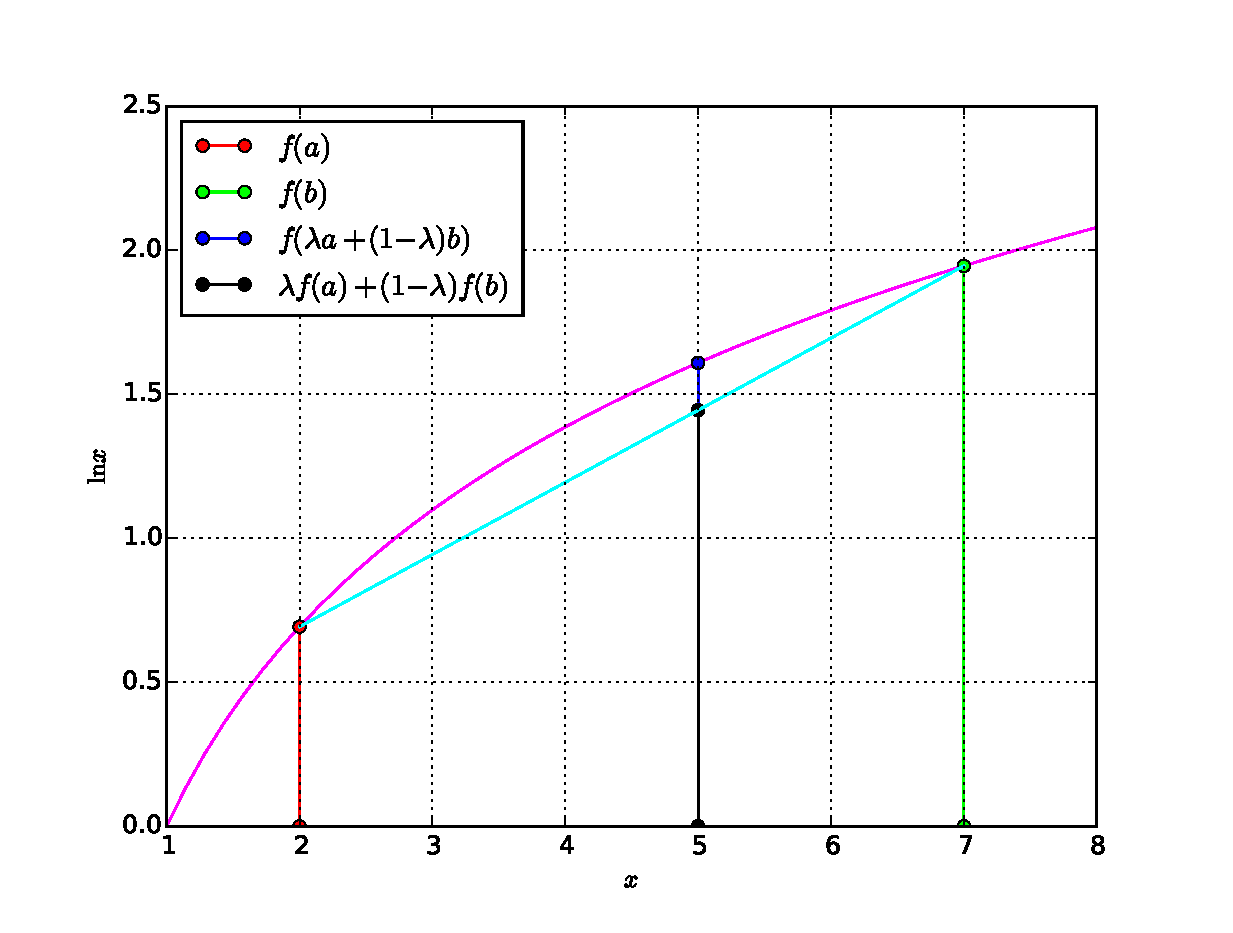
\includegraphics[width=\columnwidth]{./manual/figs/1.1.eps}
\caption{ $\ln x$ versus $x$}.
\label{fig.1.1}	
\end{figure}
%
\item
Modify the above python script as follows to plot the parabola $f(x) = x^2$. Is it convex or concave?

\begin{lstlisting}
wget https://raw.githubusercontent.com/gadepall/optimization/master/manual/codes/1.2.py
\end{lstlisting}
%
\begin{figure}[!ht]
\centering
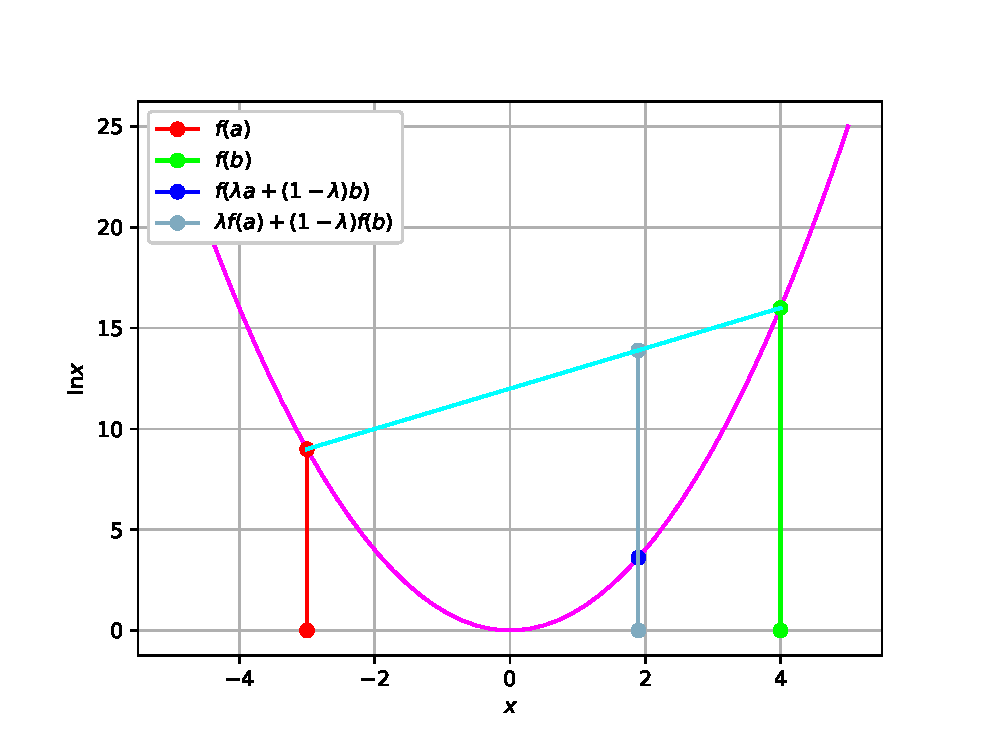
\includegraphics[width=\columnwidth]{./manual/figs/1.2.eps}
\caption{ $x^2$ versus $x$}.
\label{fig.1.2}	
\end{figure}
%
\item
Execute the following script to obtain Fig. \ref{fig.1.3}. Comment.

%
\begin{lstlisting}
wget https://raw.githubusercontent.com/gadepall/optimization/master/manual/codes/1.3.py
\end{lstlisting}

%
\begin{figure}[!ht]
\centering
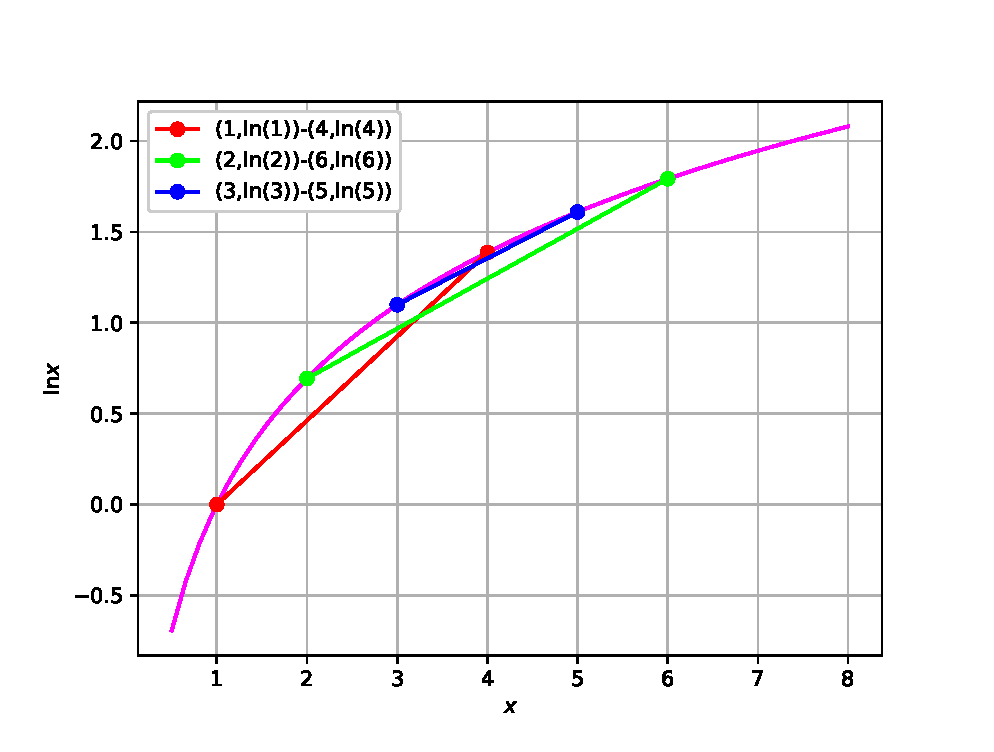
\includegraphics[width=\columnwidth]{./manual/figs/1.3.eps}
\caption{ Segments are below the curve}.
\label{fig.1.3}	
\end{figure}
%
\item
Modify the script in the previous problem for $f(x) = x^2$.  What can you conclude?

\item
Let 
\begin{equation}
f(\mathbf{x}) = x_1x_2, \quad \mathbf{x} \in \mathbf{R}^2
\end{equation}
Sketch $f(\mathbf{x})$ and deduce whether it is convex.
\item Show that 
\begin{equation}
f(\mathbf{x}) = \vec{x}^T\vec{V}\vec{x} 
\end{equation}
%
and find $\vec{V}$.
\item Show that 
\begin{equation}
\frac{1}{2}\nabla^2f(\mathbf{x}) = \vec{V}
\end{equation}

\item Use \eqref{ch1_convex_def} to examine the convexity of $f(\vec{x})$.
\item How can you deduce the convexity of $f(\vec{x})$ using the eigenvalues of $\vec{V}$?

\end{enumerate}
%
\section{Gradient Descent Method}
Consider the problem of finding the square root of a number $c$.  This can be expressed as the equation
%
\begin{equation}
\label{eq:root}
x^2 -c= 0
\end{equation}
%
\begin{enumerate}[label=\thesection.\arabic*,ref=\thesection.\theenumi]

\item
Sketch the function for different values of $c$
%
\begin{equation}
f(x)= x^{3}-3xc
\end{equation}
%
and comment upon its convexity.

\item
Show that \eqref{eq:root} results from
\begin{align}
\min_{x}f(x)= x^{3}-3xc
\end{align}

\item
Find a numerical solution for \eqref{eq:root}.

\solution
A numerical solution for \eqref{eq:root} is obtained as
%
\begin{align}
x_{n+1}&=x_{n}-\mu f^{\prime}\brak{x}
\\
&=x_{n} -\mu \brak{3x_n^{2}-3c}
\label{eq:gradient}
\end{align}

%\begin{align}
%x_{n+1}&=x_{n}-{\frac {f(x_{n})}{f^{\prime}(x_{n})}}
%\\
%&=x_{n} -\frac{x^2_{n}-c}{2x_n} 
%\\
%&=\frac{1}{2}\sbrak{x_{n} +\frac{c}{x_n} }
%\label{eq:newton}
%\end{align}
%
where $x_0$ is an inital guess.
%
\item
Write a program to implement \eqref{eq:gradient}.

%
\solution Download and execute
\begin{lstlisting}
wget 
https://raw.githubusercontent.com/gadepall/optimization/master/manual/codes/square_root.py
\end{lstlisting}
\end{enumerate}
%\section{Convex Optimization}
%\section{Lagrange Multipliers}
\begin{enumerate}[label=\thesection.\arabic*,ref=\thesection.\theenumi]

\item
	\label{convex_code}
Find
\begin{align}
\label{eq2_1_circ}
	\min_{\mbf{x}}f\brak{\mbf{x}} = \norm{\vec{x}-\myvec{8\\6}}^2 = r^2 \\
\text{s.t.} \quad 	g\brak{\mbf{x}} = \myvec{1 & 1}\vec{x} - 9 = 0\label{eq2_1_line}
%	\quad g\brak{\mbf{x}} = x_1 + x_2 - 9 = 0
\end{align}
by plotting the circles $f\brak{\vec{x}}$
%
%\begin{equation}
% \norm{\vec{x}-\myvec{8\\6}}^2 =r^2
%%(x_1-8)^2 + (x_2-6)^2 = r^2
%\end{equation}
%
% $\mbf{x}= \myvec{x_1\\x_2}$, 
for different values of $r$ along with the line $g\brak{\mbf{x}}$.
%
%\begin{equation}
%\label{eq2_1_line}
%g\brak{\mbf{x}} = \myvec{1 & 1}\vec{x} - 9 = 0
%\end{equation} 
%
\\
\solution 
The following code plots Fig. \ref{fig.2.1}	

%	
\begin{lstlisting}
wget https://raw.githubusercontent.com/gadepall/optimization/master/manual/codes/2.1.py
\end{lstlisting}

%
\begin{figure}[!ht]
\centering
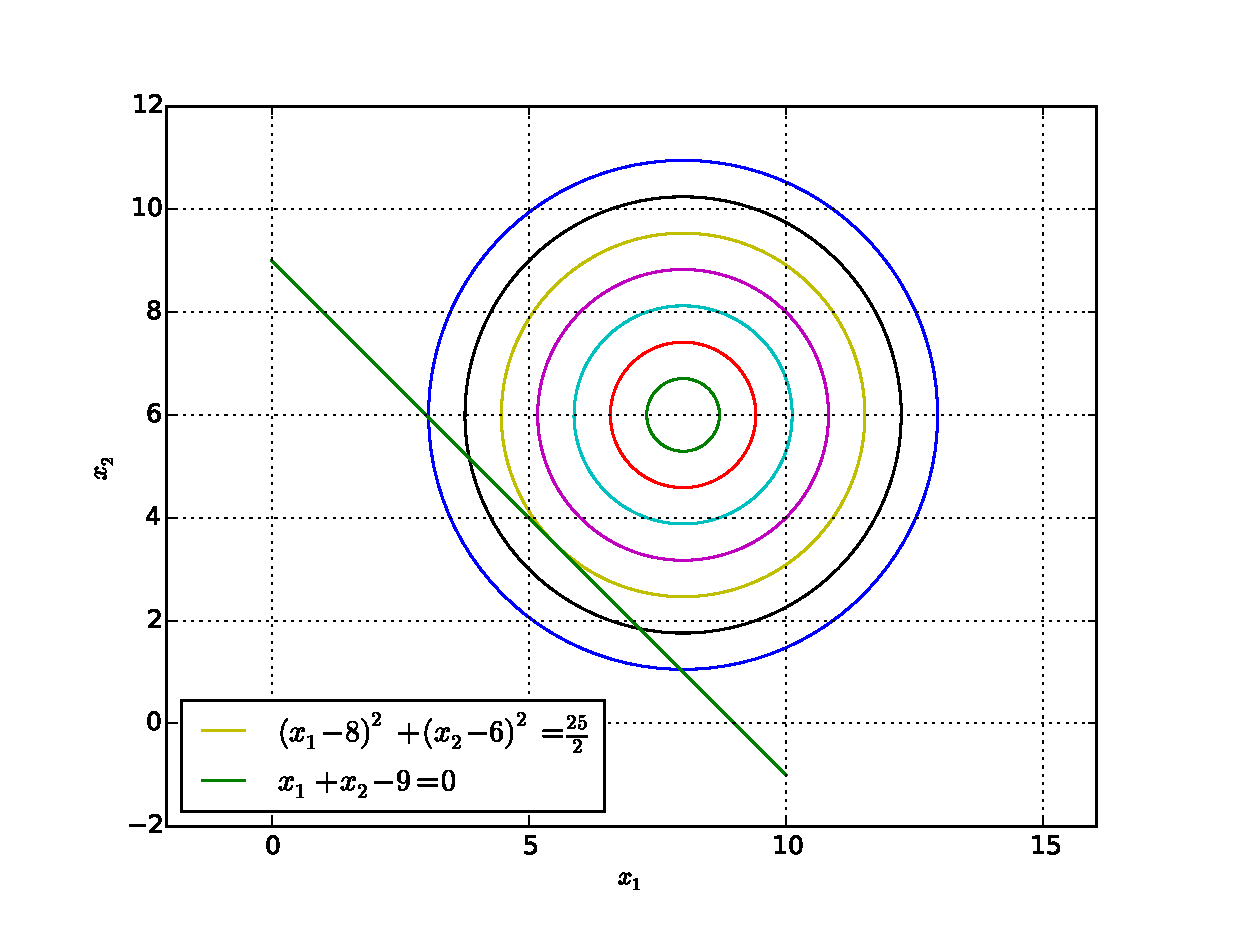
\includegraphics[width=\columnwidth]{./manual/figs/2.1.eps}
\caption{ Finding $ \displaystyle \min_{\mbf{x}}f\brak{\mbf{x}}$}.
\label{fig.2.1}	
\end{figure}
%
\item Show that 
\begin{align}
\min r = \frac{5}{\sqrt{2}}
\end{align}
%Obtain a theoretical solution for problem \ref{convex_code} 
%%using coordinate geometry.
%
%\solution 
%From \eqref{eq2_1_line} and \eqref{eq2_1_circ}, 
%%
%\begin{align}
%r^2 & = (x_1-8)^2 + (3- x_1)^2 \\
%&= 2 x_1^2 - 22 x_1 + 73 \\
%\Rightarrow r^2 &= \frac{\brak{2x_1-11}^2 + 5^2}{2}
%\end{align}
%%
%which is minium when $x_1 = \frac{11}{2}, x_2 = \frac{7}{2}$.  The minimum value is $\frac{25}{2}$ and 
%the radius $r = \frac{5}{\sqrt{2}}$.
\item Show that 
\begin{align}
\nabla g(\vec{x}) = \myvec{1 \\ 1}
\end{align}
where
\begin{equation}
\nabla =  
\begin{pmatrix}
\frac{\partial}{\partial x_1} \\
\frac{\partial}{\partial x_2} 
\end{pmatrix}
\end{equation}

\item Show that 
\begin{align}
\nabla f(\vec{x}) = 2\cbrak{\vec{x}-\myvec{8 \\ 6}}
\end{align}
\item From Fig. \ref{fig.2.1}, show that 
\begin{align}
\label{eq:normal}
\nabla f(\vec{p}) = \lambda \nabla g(\vec{p}),
\end{align}
%
where $\vec{p}$ is the point of contact.
\item Use \eqref{eq:normal} and $\vec{g(p)}=0$ from \eqref{eq2_1_line} to obtain $\vec{p}$.
\item
\label{lagrange}
	Define 
	\begin{equation}
	\label{lagrangian}
	L\brak{\mbf{x},\lambda} = f\brak{\mbf{x}} - \lambda g\brak{\mbf{x}}%, \quad \lambda > 0
	\end{equation}
and show that $\vec{p}$ can also be obtained by 
solving the equations
%
\begin{align}
\nabla L\brak{\mbf{x},\lambda} &= 0.
\label{tangent}
\end{align}
%
What is the sign of $\lambda$?  $L$ is known as the Lagrangian and the above technique is known as the Method of Lagrange Multipliers.

\solution
%From \eqref{eq2_1_line} and \eqref{eq2_1_circ}, 
%%
%\begin{align}
%L\brak{\mbf{x},\lambda} &= (x_1-8)^2 + (x_2-6)^2 - \lambda \brak{x_1 + x_2 - 9} \\
%\Rightarrow \nabla L\brak{\mbf{x},\lambda}  & = 
%\begin{pmatrix}
%2x_1  - 16 - \lambda \\
%2x_2 - 12 - \lambda \\
%x_1 + x_2 -9
%\end{pmatrix}
%\\
%&=
%\begin{pmatrix}
%2 &0 & - 1 \\
%0 &2 & - 1 \\
%1 & 1 & 0 
%\end{pmatrix}
%\begin{pmatrix}
%x_1 \\
%x_2 \\
%\lambda
%\end{pmatrix}
%= 
%\begin{pmatrix}
%16 \\
% 12 \\
%9
%\end{pmatrix}
%=
%0 
%\\
%\Rightarrow 
%\begin{pmatrix}
%x_1 \\
%x_2 \\
%\lambda
%\end{pmatrix}
%&= 
%\begin{pmatrix}
%\frac{11}{2} \\
% \frac{7}{2} \\
%-5
%\end{pmatrix}
%\end{align}
%%
%using the following python script.  Note that this method yields the same result as the previous exercises.  Thus, $\lambda$ is negative.
%	
\begin{lstlisting}
wget https://raw.githubusercontent.com/gadepall/optimization/master/manual/codes/2.3.py
\end{lstlisting}
\end{enumerate}
%\subsection{Inequality Constraints}

%
\item
\label{ch2_constraint}
Modify the code in problem \ref{convex_code} to find a graphical solution for minimising
\begin{align}
f\brak{\mbf{x}} 
%= (x_1-8)^2 + (x_2-6)^2
\end{align}
with constraint
\begin{align}
%\label{convex-constraint}
g\brak{\mbf{x}} \geq 0
%= x_1 + x_2 - 9 
\end{align}

\solution 
This problem reduces to finding the radius of the smallest circle in the shaded area in Fig. \ref{fig.2.4} .  It is clear that this radius is 0.
%	
\begin{lstlisting}
manual/codes/2.4.py
\end{lstlisting}

%
\begin{figure}[!ht]
\centering
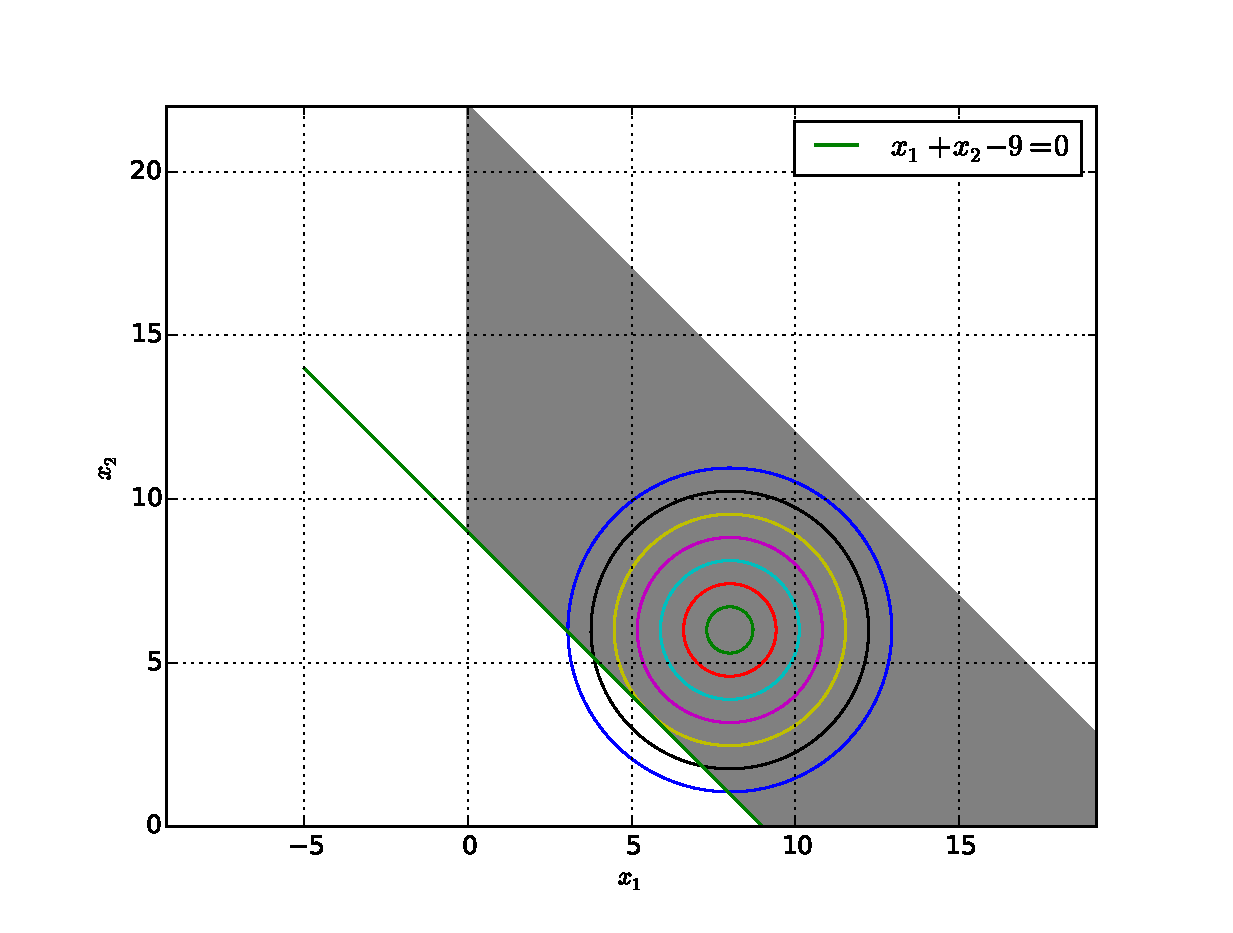
\includegraphics[width=\columnwidth]{./manual/figs/2.4.eps}
\caption{ Smallest circle in the shaded region is a point.}
\label{fig.2.4}	
\end{figure}
%
\item
\label{ch2_lagrange_fail}
Now use the method of Lagrange multipliers to solve  problem \ref{ch2_constraint} and compare with the graphical solution.  Comment.

%
\solution Using the method of Lagrange multipliers, the solution is the same as the one obtained in  problem \ref{ch2_constraint}, which is different from the graphical solution.  This means that the Lagrange multipliers method cannot be applied blindly.
\item
Repeat problem \ref{ch2_lagrange_fail} by keeping 
 $\lambda=0$.   Comment.

\solution Keeping $\lambda = 0$ results in $\vec{x}=\myvec{ 8\\ 6}$, which is the correct solution.  The minimum value of $f\brak{\mbf{x}}$ without any constraints lies in the region $g\brak{\mbf{x}} = 0$.  In this case, $\lambda = 0$.  
%
%
\item
\label{ch2_constraint_border}
Find a graphical solution for minimising
\begin{align}
f\brak{\mbf{x}}
% = (x_1-8)^2 + (x_2-6)^2
\end{align}
with constraint
\begin{align}
%\label{convex-constraint}
g\brak{\mbf{x}} \leq 0
%= x_1 + x_2 - 9 .
\end{align}
Summarize your observations.

%
\solution In Fig. \ref{fig.2.7}, the shaded region represents the constraint.  Thus, the solution is the same as the one in problem \ref{ch2_constraint}. This implies that the method of
Lagrange multipliers can be used to solve the optimization problem with this inequality constraint as well.  Table \ref{table.2.7} summarizes the conditions for this based on the observations so far.
\begin{lstlisting}
manual/codes/2.7.py
\end{lstlisting}

%
\begin{figure}[!ht]
\centering
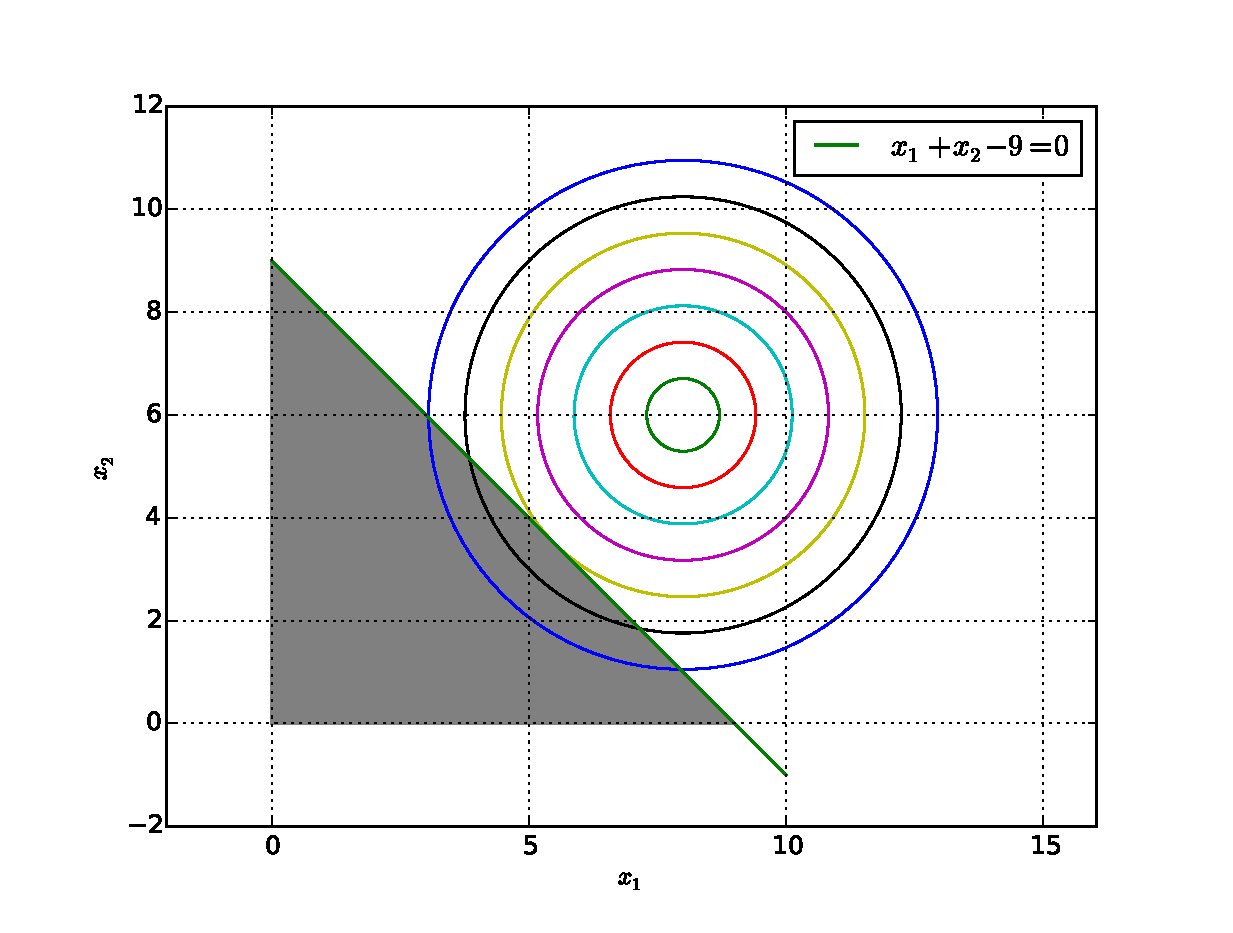
\includegraphics[width=\columnwidth]{./manual/figs/2.7.eps}
\caption{ Finding $ \displaystyle \min_{\mbf{x}}f\brak{\mbf{x}}$.}
\label{fig.2.7}	
\end{figure}
%%%%%%%%%%%%%%%%%%%%%%%%%%%%%%%%%%%%%%%%%%%%%%%%%%%%%%%%%%%%%%%%%%%%%%
%%                                                                  %%
%%  This is the header of a LaTeX2e file exported from Gnumeric.    %%
%%                                                                  %%
%%  This file can be compiled as it stands or included in another   %%
%%  LaTeX document. The table is based on the longtable package so  %%
%%  the longtable options (headers, footers...) can be set in the   %%
%%  preamble section below (see PRAMBLE).                           %%
%%                                                                  %%
%%  To include the file in another, the following two lines must be %%
%%  in the including file:                                          %%
%%        \def\inputGnumericTable{}                                 %%
%%  at the beginning of the file and:                               %%
%%        \input{name-of-this-file.tex}                             %%
%%  where the table is to be placed. Note also that the including   %%
%%  file must use the following packages for the table to be        %%
%%  rendered correctly:                                             %%
%%    \usepackage[latin1]{inputenc}                                 %%
%%    \usepackage{color}                                            %%
%%    \usepackage{array}                                            %%
%%    \usepackage{longtable}                                        %%
%%    \usepackage{calc}                                             %%
%%    \usepackage{multirow}                                         %%
%%    \usepackage{hhline}                                           %%
%%    \usepackage{ifthen}                                           %%
%%  optionally (for landscape tables embedded in another document): %%
%%    \usepackage{lscape}                                           %%
%%                                                                  %%
%%%%%%%%%%%%%%%%%%%%%%%%%%%%%%%%%%%%%%%%%%%%%%%%%%%%%%%%%%%%%%%%%%%%%%



%%  This section checks if we are begin input into another file or  %%
%%  the file will be compiled alone. First use a macro taken from   %%
%%  the TeXbook ex 7.7 (suggestion of Han-Wen Nienhuys).            %%
\def\ifundefined#1{\expandafter\ifx\csname#1\endcsname\relax}


%%  Check for the \def token for inputed files. If it is not        %%
%%  defined, the file will be processed as a standalone and the     %%
%%  preamble will be used.                                          %%
\ifundefined{inputGnumericTable}

%%  We must be able to close or not the document at the end.        %%
	\def\gnumericTableEnd{\end{document}}


%%%%%%%%%%%%%%%%%%%%%%%%%%%%%%%%%%%%%%%%%%%%%%%%%%%%%%%%%%%%%%%%%%%%%%
%%                                                                  %%
%%  This is the PREAMBLE. Change these values to get the right      %%
%%  paper size and other niceties.                                  %%
%%                                                                  %%
%%%%%%%%%%%%%%%%%%%%%%%%%%%%%%%%%%%%%%%%%%%%%%%%%%%%%%%%%%%%%%%%%%%%%%

	\documentclass[12pt%
			  %,landscape%
                    ]{report}
       \usepackage[latin1]{inputenc}
       \usepackage{fullpage}
       \usepackage{color}
       \usepackage{array}
       \usepackage{longtable}
       \usepackage{calc}
       \usepackage{multirow}
       \usepackage{hhline}
       \usepackage{ifthen}

	\begin{document}


%%  End of the preamble for the standalone. The next section is for %%
%%  documents which are included into other LaTeX2e files.          %%
\else

%%  We are not a stand alone document. For a regular table, we will %%
%%  have no preamble and only define the closing to mean nothing.   %%
    \def\gnumericTableEnd{}

%%  If we want landscape mode in an embedded document, comment out  %%
%%  the line above and uncomment the two below. The table will      %%
%%  begin on a new page and run in landscape mode.                  %%
%       \def\gnumericTableEnd{\end{landscape}}
%       \begin{landscape}


%%  End of the else clause for this file being \input.              %%
\fi

%%%%%%%%%%%%%%%%%%%%%%%%%%%%%%%%%%%%%%%%%%%%%%%%%%%%%%%%%%%%%%%%%%%%%%
%%                                                                  %%
%%  The rest is the gnumeric table, except for the closing          %%
%%  statement. Changes below will alter the table's appearance.     %%
%%                                                                  %%
%%%%%%%%%%%%%%%%%%%%%%%%%%%%%%%%%%%%%%%%%%%%%%%%%%%%%%%%%%%%%%%%%%%%%%

\providecommand{\gnumericmathit}[1]{#1} 
%%  Uncomment the next line if you would like your numbers to be in %%
%%  italics if they are italizised in the gnumeric table.           %%
%\renewcommand{\gnumericmathit}[1]{\mathit{#1}}
\providecommand{\gnumericPB}[1]%
{\let\gnumericTemp=\\#1\let\\=\gnumericTemp\hspace{0pt}}
 \ifundefined{gnumericTableWidthDefined}
        \newlength{\gnumericTableWidth}
        \newlength{\gnumericTableWidthComplete}
        \newlength{\gnumericMultiRowLength}
        \global\def\gnumericTableWidthDefined{}
 \fi
%% The following setting protects this code from babel shorthands.  %%
 \ifthenelse{\isundefined{\languageshorthands}}{}{\languageshorthands{english}}
%%  The default table format retains the relative column widths of  %%
%%  gnumeric. They can easily be changed to c, r or l. In that case %%
%%  you may want to comment out the next line and uncomment the one %%
%%  thereafter                                                      %%
\providecommand\gnumbox{\makebox[0pt]}
%%\providecommand\gnumbox[1][]{\makebox}

%% to adjust positions in multirow situations                       %%
\setlength{\bigstrutjot}{\jot}
\setlength{\extrarowheight}{\doublerulesep}

%%  The \setlongtables command keeps column widths the same across  %%
%%  pages. Simply comment out next line for varying column widths.  %%
\setlongtables

\setlength\gnumericTableWidth{%
	53pt+%
	58pt+%
	55pt+%
0pt}
\def\gumericNumCols{3}
\setlength\gnumericTableWidthComplete{\gnumericTableWidth+%
         \tabcolsep*\gumericNumCols*2+\arrayrulewidth*\gumericNumCols}
\ifthenelse{\lengthtest{\gnumericTableWidthComplete > \linewidth}}%
         {\def\gnumericScale{\ratio{\linewidth-%
                        \tabcolsep*\gumericNumCols*2-%
                        \arrayrulewidth*\gumericNumCols}%
{\gnumericTableWidth}}}%
{\def\gnumericScale{1}}

%%%%%%%%%%%%%%%%%%%%%%%%%%%%%%%%%%%%%%%%%%%%%%%%%%%%%%%%%%%%%%%%%%%%%%
%%                                                                  %%
%% The following are the widths of the various columns. We are      %%
%% defining them here because then they are easier to change.       %%
%% Depending on the cell formats we may use them more than once.    %%
%%                                                                  %%
%%%%%%%%%%%%%%%%%%%%%%%%%%%%%%%%%%%%%%%%%%%%%%%%%%%%%%%%%%%%%%%%%%%%%%

\ifthenelse{\isundefined{\gnumericColA}}{\newlength{\gnumericColA}}{}\settowidth{\gnumericColA}{\begin{tabular}{@{}p{53pt*\gnumericScale}@{}}x\end{tabular}}
\ifthenelse{\isundefined{\gnumericColB}}{\newlength{\gnumericColB}}{}\settowidth{\gnumericColB}{\begin{tabular}{@{}p{58pt*\gnumericScale}@{}}x\end{tabular}}
\ifthenelse{\isundefined{\gnumericColC}}{\newlength{\gnumericColC}}{}\settowidth{\gnumericColC}{\begin{tabular}{@{}p{55pt*\gnumericScale}@{}}x\end{tabular}}

\begin{table}[!h]
	\caption{Summary of conditions.} 
	\centering
\begin{tabular}[c]{%
	b{\gnumericColA}%
	b{\gnumericColB}%
	b{\gnumericColC}%
	}

%%%%%%%%%%%%%%%%%%%%%%%%%%%%%%%%%%%%%%%%%%%%%%%%%%%%%%%%%%%%%%%%%%%%%%
%%  The longtable options. (Caption, headers... see Goosens, p.124) %%            \\	%
 %\hline	% Across the top of the table.
%%  The rest of these options are table rows which are placed on    %%
%%  the first, last or every page. Use \multicolumn if you want.    %%

%%  Header for the first page.                                      %%
%	\multicolumn{3}{c}{The First Header} \\ \hline 
%	\multicolumn{1}{c}{colTag}	%Column 1
%	&\multicolumn{1}{c}{colTag}	%Column 2
%	&\multicolumn{1}{c}{colTag}	\\ \hline %Last column
%	\endfirsthead

%%  The running header definition.                                  %%
%	\hline
%	\multicolumn{3}{l}{\ldots\small\slshape continued} \\ \hline
%	\multicolumn{1}{c}{colTag}	%Column 1
%	&\multicolumn{1}{c}{colTag}	%Column 2
%	&\multicolumn{1}{c}{colTag}	\\ \hline %Last column
%	\endhead

%%  The running footer definition.                                  %%
%	\hline
%	\multicolumn{3}{r}{\small\slshape continued\ldots} \\
%	\endfoot

%%  The ending footer definition.                                   %%
%	\multicolumn{3}{c}{That's all folks} \\ \hline 
%	\endlastfoot
%%%%%%%%%%%%%%%%%%%%%%%%%%%%%%%%%%%%%%%%%%%%%%%%%%%%%%%%%%%%%%%%%%%%%%

\hhline{|-|-|-}
	 \multicolumn{1}{|p{\gnumericColA}|}%
	{\gnumericPB{\centering}\textbf{Cost}}
	&\multicolumn{1}{p{\gnumericColB}|}%
	{\gnumericPB{\centering}\textbf{Constraint}}
	&\multicolumn{1}{p{\gnumericColC}|}%
	{\gnumericPB{\centering}\textbf{$\lambda$}}
\\
\hhline{|---|}
	 \multicolumn{1}{|p{\gnumericColA}|}%
	{\setlength{\gnumericMultiRowLength}{0pt}%
	 \addtolength{\gnumericMultiRowLength}{\gnumericColA}%
	 \multirow{3}[1]{\gnumericMultiRowLength}{\parbox{\gnumericMultiRowLength}{%
	 \gnumericPB{\centering}$f\brak{\mbf{x}}$}}}
	&\multicolumn{1}{p{\gnumericColB}|}%
	{\gnumericPB{\centering}$g\brak{\mbf{x}} = 0$}
	&\multicolumn{1}{p{\gnumericColC}|}%
	{\gnumericPB{\centering} $<$ 0}
\\
\hhline{~|--|}
	 \multicolumn{1}{|p{\gnumericColA}|}%
	{}
	&\multicolumn{1}{p{\gnumericColB}|}%
	{\gnumericPB{\centering}$g\brak{\mbf{x}} \geq 0 $}
	&\multicolumn{1}{p{\gnumericColC}|}%
	{\gnumericPB{\centering}0}
\\
\hhline{~|--|}
	 \multicolumn{1}{|p{\gnumericColA}|}%
	{}
	&\multicolumn{1}{p{\gnumericColB}|}%
	{\gnumericPB{\centering}$g\brak{\mbf{x}}\leq 0 $}
	&\multicolumn{1}{p{\gnumericColC}|}%
	{\gnumericPB{\centering} $<$ 0}
\\
\hhline{|-|-|-|}
\end{tabular}
\label{table.2.7}
\end{table}

\ifthenelse{\isundefined{\languageshorthands}}{}{\languageshorthands{\languagename}}
\gnumericTableEnd

%
\item
\label{ch2_prob_upper}
Find a graphical solution for 	 
	 \begin{align}
	 \label{ch2_second_min}
	\min_{\mbf{x}} f\brak{\mbf{x}} = \norm{\vec{x}-\myvec{8\\6}}^2
	 \end{align}
	 with constraint
	 \begin{align}
	 \label{ch2_second_const}
	 g\brak{\mbf{x}} = \myvec{1 & 1}\vec{x} - 18 = 0
	 \end{align}
	 
%
\solution
%	
\begin{lstlisting}
manual/codes/2.8.py
\end{lstlisting}

%
\begin{figure}[!ht]
\centering
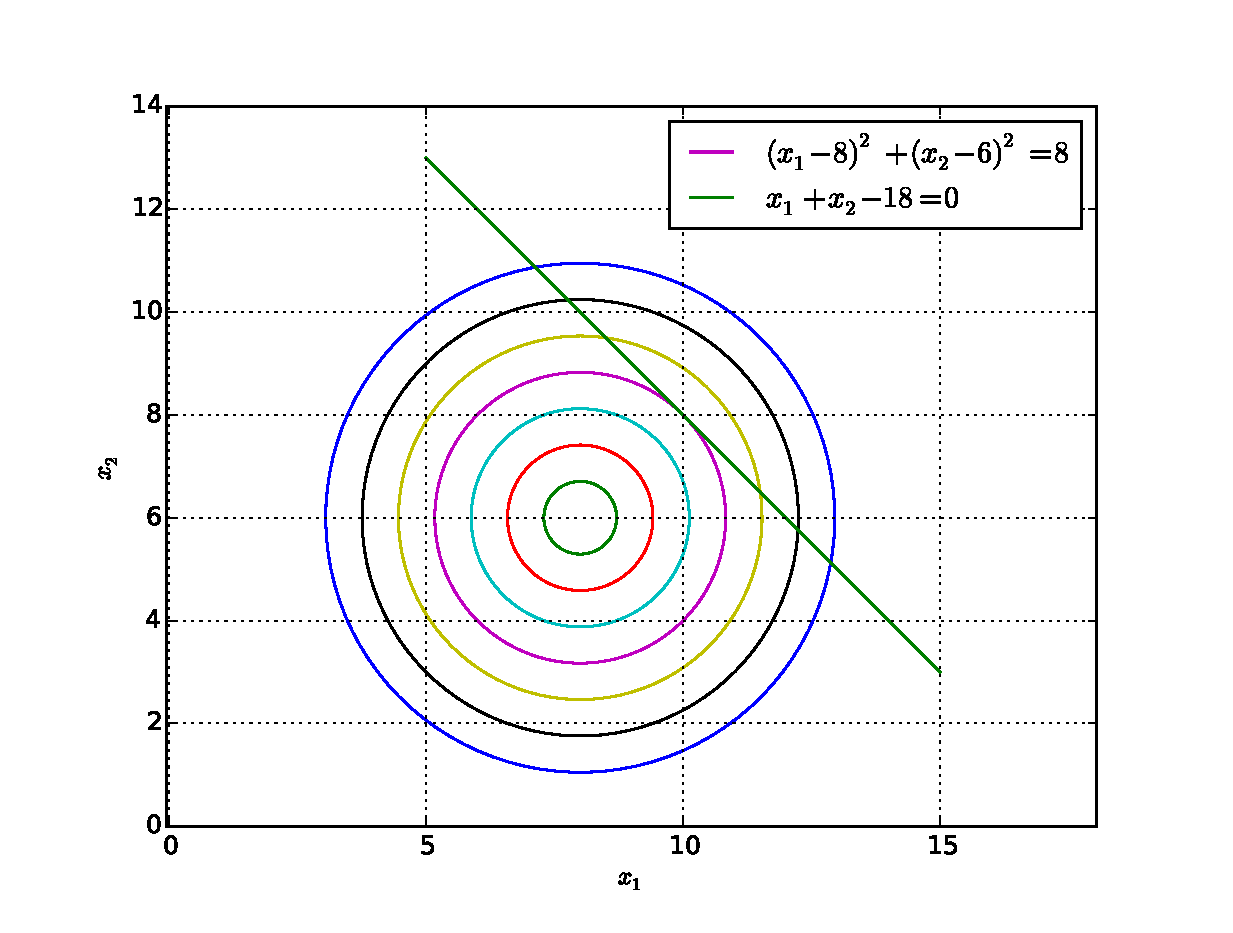
\includegraphics[width=\columnwidth]{./manual/figs/2.8.eps}
\caption{ Finding $ \displaystyle \min_{\mbf{x}}f\brak{\mbf{x}}$.}
\label{fig.2.8}	
\end{figure}
%
\item
Repeat problem \ref{ch2_prob_upper} using the method of Lagrange mutipliers.  What is the sign of $\lambda$?

%
\solution
%From \eqref{ch2_second_min} and \eqref{ch2_second_const}, 
%%
%\begin{align}
%L\brak{\mbf{x},\lambda} &= (x_1-8)^2 + (x_2-6)^2 - \lambda \brak{x_1 + x_2 - 18} \\
%\Rightarrow \nabla L\brak{\mbf{x},\lambda}  & = 
%\begin{pmatrix}
%2x_1  - 16 - \lambda \\
%2x_2 - 12 - \lambda \\
%x_1 + x_2 -18
%\end{pmatrix}
%\\
%&=
%\begin{pmatrix}
%2 &0 & - 1 \\
%0 &2 & - 1 \\
%1 & 1 & 0 
%\end{pmatrix}
%\begin{pmatrix}
%x_1 \\
%x_2 \\
%\lambda
%\end{pmatrix}
%= 
%\begin{pmatrix}
%16 \\
% 12 \\
%18
%\end{pmatrix}
%=
%0 
%\\
%\Rightarrow 
%\begin{pmatrix}
%x_1 \\
%x_2 \\
%\lambda
%\end{pmatrix}
%&= 
%\begin{pmatrix}
%10 \\
% 8 \\
%4
%\end{pmatrix}
%\end{align}
%%
Using the following python script, $\lambda$ is positive and the minimum value of $f$ is 8.
%	
\begin{lstlisting}
manual/codes/2.9.py
\end{lstlisting}

%
%
\item
\label{ch2_prob_upper_cond}
Solve
	 \begin{align}
%	 \label{ch2_second_min}
	\min_{\mbf{x}} f\brak{\mbf{x}} 
%= (x_1-8)^2 + (x_2-6)^2
	 \end{align}
	 with constraint
	 \begin{align}
%	 \label{ch2_second_const}
	 g\brak{\mbf{x}} 
%= x_1 + x_2 - 18 
\geq 0 
	 \end{align}
	 
%
\solution Since the unconstrained solution is outside the region $g\brak{\mbf{x}} \geq 0$, the solution is the same as the one in problem \ref{ch2_prob_upper}.
%
\item
Based on the problems so far, generalise the Lagrange multipliers method for 
%
	 \begin{align}
	 \label{ch2_lagrange_ineq}
	\min_{\mbf{x}} f\brak{\mbf{x}} , \quad 
	 g\brak{\mbf{x}}  \geq 0 
	 \end{align}
%

%
\solution
Considering $L\brak{\mbf{x},\lambda} = f\brak{\mbf{x}} - \lambda g\brak{\mbf{x}}$, for $g\brak{\mbf{x}} = \myvec{1 & 1}\vec{x} - 18 \geq 0$ we found $\lambda > 0 $ and for $g\brak{\mbf{x}} = \myvec{1 & 1}\vec{x} - 9 \leq 0, \lambda < 0$. A single condition can be obtained by framing the optimization problem as
%
	 \begin{align}
	 \label{ch2_lagrange_ineq_summary}
	\min_{\mbf{x}} f\brak{\mbf{x}} , \quad 
	 g\brak{\mbf{x}}  \leq 0 
	 \end{align}
%
with the Lagrangian
%
\begin{equation}
%\label{ch2_kkt_necessary}
L\brak{\mbf{x},\lambda} = f\brak{\mbf{x}} + \lambda g\brak{\mbf{x}}, %\quad  \lambda > 0,  g\brak{\mbf{x}} \leq 0.
\end{equation}
%
provided
%
\begin{equation}
\label{ch2_kkt_necessary}
\nabla L\brak{\mbf{x},\lambda} = 0 \Rightarrow \lambda > 0
\end{equation}
else, $\lambda = 0$.
\end{enumerate}
\begin{enumerate}[label=\thesection.\arabic*,ref=\thesection.\theenumi]
%\subsection{Karush Kuhn-Tucker Conditions}
\item
Solve
 \begin{align}
 \label{ch2_kkt_problem}
\min_{\mbf{x}} f\brak{\mbf{x}} = \vec{x}^T\myvec{4 & 0 \\0 & 2}\vec{x}
%4x_1^2 + 2x_2^2
 \end{align}
 with constraints
 \begin{align}
 g_1\brak{\mbf{x}} = \myvec{3 & 1}\vec{x}-8 = 0\\
 g_2 \brak{\mbf{x}}= 15 - \myvec{2 & 4}\vec{x} \geq 0
 \end{align}
 
%
\solution Considering the Lagrangian
%
\begin{align}
%L\brak{\mbf{x},\lambda} &= f\brak{\mbf{x}} + \lambda g_1\brak{\mbf{x}} - \mu g_2\brak{\mbf{x}} \\
% &= 4x_1^2 + 2x_2^2 + \lambda \brak{3x_1 + x_2-8} 
% \nonumber \\
% &\,-\mu\brak{15 - 2x_1 - 4x_2},\\
 \nabla L\brak{\mbf{x},\lambda, \mu}  %& = 
%\begin{pmatrix}
%8x_1 + 3 \lambda  +2 \mu  \\
%4x_2 + \lambda + 4 \mu \\
%3x_1 + x_2 -8 \\
% - 2x_1 - 4x_2 + 15
%\end{pmatrix}
= 0
\end{align}
%
resulting in the matrix equation
%
\begin{align}
\Rightarrow 
\begin{pmatrix}
8 &0 & 3 & 2\\
0 &4 & 1 & 4 \\
3 & 1 & 0 &0  \\
2 & 4 & 0 & 0
\end{pmatrix}
\begin{pmatrix}
x_1 \\
x_2 \\
\lambda
\\
\mu
\end{pmatrix}
&=
\begin{pmatrix}
0 \\
0 \\
8 \\
15
\end{pmatrix}
\\
\Rightarrow 
\begin{pmatrix}
x_1 \\
x_2 \\
\lambda
\\
\mu
\end{pmatrix}
&= 
\begin{pmatrix}
1.7 \\
 2.9 \\
-3.12 \\
-2.12
\end{pmatrix}
\end{align}
%
using the following python script.  The (incorrect) graphical solution is available in Fig. \ref{fig.2.12}
%	
\begin{lstlisting}
manual/codes/2.12.py
\end{lstlisting}

%
Note that $\mu < 0 $, contradicting the necessary condition in \eqref{ch2_kkt_necessary}. 
%
\begin{figure}[!ht]
\centering
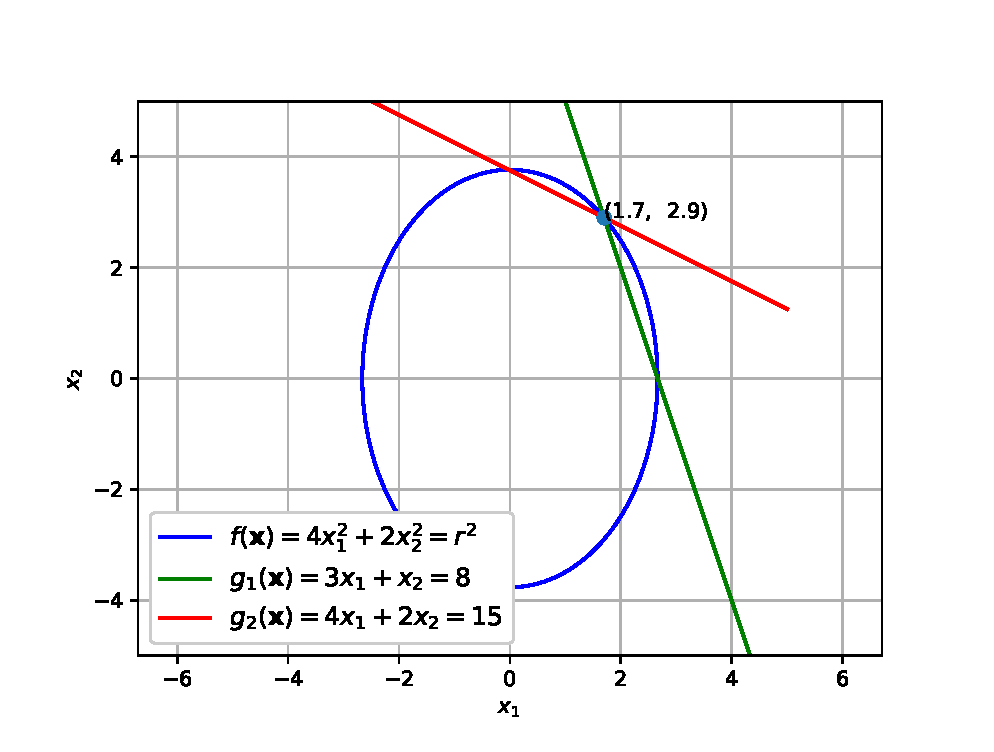
\includegraphics[width=\columnwidth]{./manual/figs/2.12_1.eps}
\caption{ Incorrect solution is at intersection of all curves $r = 5.33$}
\label{fig.2.12}	
\end{figure}
\item
Obtain the correct solution to the previous problem by considering $\mu = 0$.

\begin{figure}[!ht]
\centering
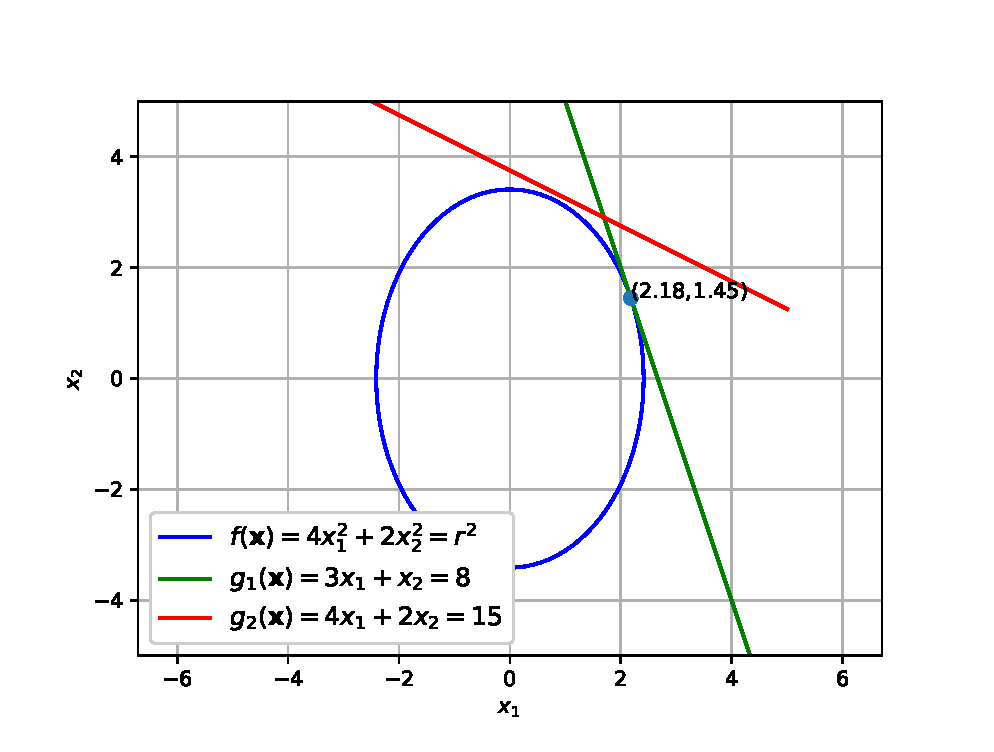
\includegraphics[width=\columnwidth]{./manual/figs/2.12_2.eps}
\caption{ Optimal solution is where $g_1(x)$ touches the curve $r = 4.82$}
\label{fig.2.13}	
\end{figure}
%
%
\item
Solve
 \begin{align}
% \label{ch2_kkt_problem}
\min_{\mbf{x}} f\brak{\mbf{x}} %= 4x_1^2 + 2x_2^2
 \end{align}
 with constraints
 \begin{align}
 g_1\brak{\mbf{x}} 
%= 3x_1 + x_2-8 
= 0\\
 g_2 \brak{\mbf{x}}
%= 15 - 2x_1 - 4x_2 
\leq 0
 \end{align}
 
%
\item
Based on whatever you have done so far,	list the steps that you would use in general for solving a convex optimization problem  like \eqref{ch2_kkt_problem}  using Lagrange Multipliers. 
These are called Karush-Kuhn-Tucker(KKT) conditions.

\solution For a problem defined by 
\begin{align}
\mbf{x^*} &= \min_{\mbf{x}}f(\mbf{x})
\\
\text{subject to } h_i(\mbf{x}) &= 0, \forall i=1,..,m
\\
\text{subject to } g_i(\mbf{x}) &\le 0, \forall i=1,..,n
\end{align}
%
the optimal solution is obtained through
%
\begin{align}
\mbf{x^*} &= \min_{\mbf{x}}L(\mbf{x}, \mbf{\lambda}, \mbf{\mu}) 
\\
&= \min_{\mbf{x}}f(\mbf{x})  + \underset{i=1}{\overset{m}{\sum}} \lambda_i h_i(\mbf{x}) + \underset{i=1}{\overset{n}{\sum}} \mu_i g_i(\mbf{x}),
\end{align}
%
using the KKT conditions
%
\begin{align}
\Rightarrow \nabla_\mbf{x} f(\mbf{x})  + \underset{i=1}{\overset{m}{\sum}} \nabla_\mbf{x} \lambda_i h_i(\mbf{x}) + \underset{i=1}{\overset{n}{\sum}} \mu_i \nabla_\mbf{x} g_i(\mbf{x}) = 0 
\\
\text{subject to }\mu_i g_i(\mbf{x}) = 0, \forall i = 1,..,n
\\
\text{and }\mu_i \ge 0, \forall i = 1,..,n
\end{align}
%
\item
	Maxmimize 
	%
	\begin{align}
	f(\mbf{x}) &= \sqrt{x_1x_2}
	\end{align}
	%
	with the constraints
	%
	\begin{align}
	x_1^2+x_2^2 &\leq 5 \\
	x_1 \geq 0, x_2 &\geq 0
	\end{align}
	%

%
\item
	\label{convex_sdp_eqiv}
	%
	Solve
	\begin{equation}
	\min_{\mbf{x}} \quad x_1 + x_2
	\end{equation}
	%	
	with the constraints
	\begin{equation}
	x_1^2 - x_1 + x_2^2 \leq 0
	\end{equation}
	%
where 
$
\mbf{x} = \begin{pmatrix}
x_1 \\
x_2
\end{pmatrix}
$

\solution 
%Using the method of Lagrange multipliers,
%%
%\begin{align}
%\label{ch2_sd_kkt}
%\nabla \cbrak{f(\mbf{x})  +  \mu g(\mbf{x}) }= 0 , \quad \mu \ge 0
%\end{align}
%%
%resulting in the equations
%%
%\begin{align}
%2x_1\mu -\mu + 1 &= 0 \\
%2x_2\mu + 1 &=0 \\
%x_1^2 -x_1 + x_2^2 &= 0 
%\end{align}
%%
%which can be simplified to obtain 
%%
%\begin{align}
%\brak{\frac{1-\mu}{2\mu}}^2 + \brak{\frac{1}{2\mu}}^2 + \frac{1-\mu}{2\mu} &= 0 \\
%\Rightarrow 1 + \mu^2 -2\mu + 1 + 2\mu\brak{1-\mu} &= 0 \\
%\Rightarrow \mu^2 =2, or \mu &= \pm \sqrt{2} 
%\end{align}
%%
%From \eqref{ch2_kkt_problem},  $\mu \ge 0 \Rightarrow  \mu = \sqrt{2}$. The desired solution is
%%
%\begin{equation}
%\mbf{x} = 
%\begin{pmatrix}
% \frac{\sqrt{2}-1}{2\sqrt{2}} \\
%-\frac{1}{2\sqrt{2}} 
%\end{pmatrix}
%\end{equation}
%
\\
{\em Graphical solution:} 
%The constraint can be expressed as
%%
%\begin{align}
%x_1^2 - x_1 + x_2^2 &\le 0 \\
%\Rightarrow \brak{x_1 - \frac{1}{2}}^2 + x_2^2 & \le \brak{\frac{1}{2}}^2
%\end{align}
%
%	
\begin{lstlisting}
manual/codes/2.15.py
\end{lstlisting}

%
%
\begin{figure}[!ht]
\centering
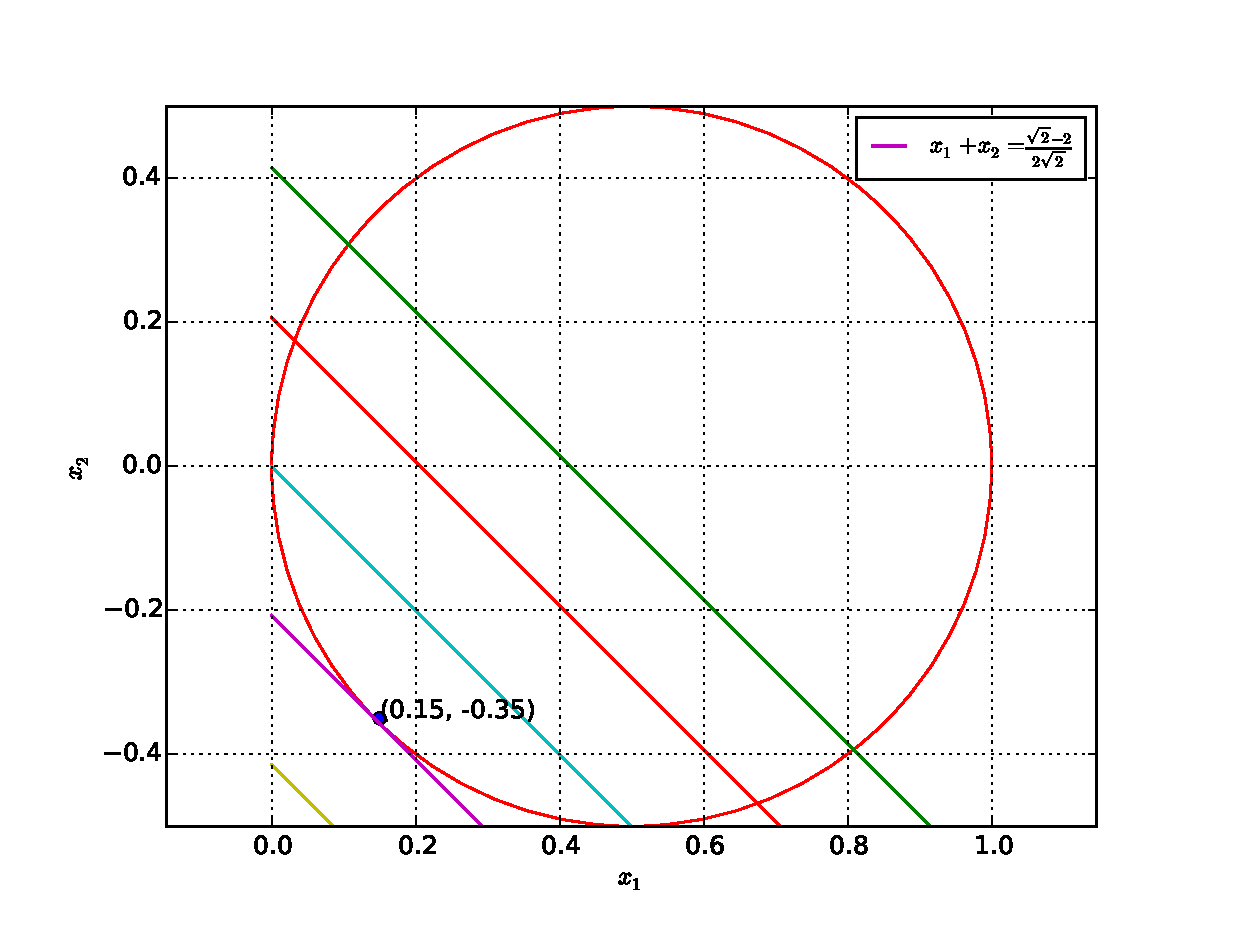
\includegraphics[width=\columnwidth]{./manual/figs/2.15.eps}
\caption{ Optimal solution is the lower tangent to the circle}
\label{fig.2.15}	
\end{figure}
%
\end{enumerate}

\section{Semi-definite Programming}
\fi
\begin{enumerate}[label=\thesection.\arabic*,ref=\thesection.\theenumi]

%\subsection{Karush Kuhn-Tucker Conditions}

\item
%
\label{ch3_convex_ch2}
The problem
\begin{equation}
\min_{\mbf{X}} x_{11} + x_{12}
\end{equation}
%	
with constraints
\begin{align}
x_{11} + x_{22} &= 1 \\	
\mbf{X}
& \succeq 0 \quad  \brak{\text{$\succeq$ means positive definite}}
\end{align}
%
where
\begin{equation}
\mbf{X}=
\begin{pmatrix}
x_{11} & x_{12} \\
x_{12} & x_{22}
\end{pmatrix} 
\end{equation}
%
is known as a semi-definite program.  Find a numerical solution to this problem. Compare with the solution 
in problem  \ref{convex_sdp_eqiv}.
\label{prob:cvxopt}

\solution The {\em cvxopt} solver needs to be used in order to find a numerical solution.  For this, the given problem has to be reformulated as
\begin{align}
&\min_{\mbf{x}}  
\begin{pmatrix}
1 & 1 & 0
\end{pmatrix}
\begin{pmatrix}
x_{11} 
\\
x_{12}
\\
x_{22}
\end{pmatrix}
\quad \text{s.t}
\\
&
\begin{pmatrix}
1 & 0 & 1
\end{pmatrix}
\begin{pmatrix}
x_{11} 
\\
x_{12}
\\
x_{22}
\end{pmatrix}
=1
\end{align}
\begin{multline}
x_{11}
\begin{pmatrix}
-1 & 0 
\\
0 & 0
\end{pmatrix}
+
x_{12}
\begin{pmatrix}
0 & -1
\\
-1 & 0
\end{pmatrix}
+x_{22}
\begin{pmatrix}
0 & 0 
\\
0 & -1
\end{pmatrix}
\\
\preceq 
\begin{pmatrix}
0 & 0 
\\
0 & 0
\end{pmatrix}.
\end{multline}
%
The following script provides the solution to this problem.
\begin{lstlisting}
wget https://raw.githubusercontent.com/gadepall/optimization/master/manual/codes/3.1.py
\end{lstlisting}
%
\item
Frame Problem \ref{prob:cvxopt} in terms of matrices.

\solution
It is easy to verify that
\begin{equation}
x_{11} + x_{12} = 
\begin{pmatrix}
1 & 1
\end{pmatrix}
\mbf{X}^{T}
\begin{pmatrix}
1 
\\
0
\end{pmatrix}
\end{equation}
and
\begin{equation}
x_{11} + x_{22} = 
\begin{pmatrix}
1 & 0 & 0 & 1
\end{pmatrix}
\begin{pmatrix}
\mbf{X} & \mbf{0} \\
\mbf{0} & \mbf{X}
\end{pmatrix}
\begin{pmatrix}
1
\\
0 
\\
0
\\
1
\end{pmatrix}
\end{equation}
%
Thus, Problem \ref{prob:cvxopt} can be expressed as
\begin{equation}
\begin{split}
\min_{\mbf{X}} 
\begin{pmatrix}
1 & 1
\end{pmatrix}
\mbf{X}^{T}
\begin{pmatrix}
1 
\\
0
\end{pmatrix}
& \quad s.t
\\
\begin{pmatrix}
1 & 0 & 0 & 1
\end{pmatrix}
\begin{pmatrix}
\mbf{X} & \mbf{0} \\
\mbf{0} & \mbf{X}
\end{pmatrix}
\begin{pmatrix}
1
\\
0 
\\
0
\\
1
\end{pmatrix}
&=1,
\\
\mbf{X}
 & \succeq 0 
\end{split}
\label{prob:cvxpy}
\end{equation}
%	
\item
Solve \eqref{prob:cvxpy} using {\em cvxpy}.

%
\solution
\begin{lstlisting}
wget https://raw.githubusercontent.com/gadepall/optimization/master/manual/codes/3.1-cvx.py
\end{lstlisting}

\item
Minimize 
\begin{equation}
-x_{11} - 2x_{12} - 5x_{22}
\end{equation}
subject to
\begin{align}
\label{ch3_lin_mat_ineq_const}
2x_{11} + 3x_{12} + x_{22} &= 7 \\
x_{11} + x_{12} &\geq 1 \\
x_{11}, x_{12}, x_{22} &\geq 0 \\
\begin{pmatrix}
x_{11} & x_{12} \\
x_{12} & x_{22}
\end{pmatrix} & \succeq 0 
\end{align}
using {\em cvxpy}.

%\solution
%In this problem, there is an SDP inequality and several linear inequalities.  The linear inequalities can be combined to obtain the matrix inequality
%%
%\begin{equation}
%\label{ch3_lin_mat_ineq}
%\begin{pmatrix}
%x_{11} + x_{12}- 1 & 0  & 0 & 0\\
%0 & x_{11} & 0 & 0
%\\
%0 & 0 & x_{12} &  0
%\\
 %0 & 0 & 0 & x_{22} 
%\end{pmatrix}
 %\succeq 0 
%\end{equation}
%%
%\eqref{ch3_lin_mat_ineq} can be combined with the matrix inequality in \eqref{ch3_lin_mat_ineq_const} to obtain the composite SDP
%\begin{equation}
%\label{ch3_lin_mat_sdp_ineq}
%\begin{pmatrix}
%\begin{matrix}
%x_{11} + x_{12}- 1 & 0  & 0 & 0\\
%0 & x_{11} & 0 & 0
%\\
%0 & 0 & x_{12} &  0
%\\
 %0 & 0 & 0 & x_{22} 
%\end{matrix}
%& \mbf{0}
%\\
%\mbf{0} & \begin{matrix}
%x_{11} & x_{12} \\
%x_{12} & x_{22}
%\end{matrix}
%\end{pmatrix} 
 %\succeq 0 
%\end{equation}
%%
%For using  {\em cvxpy}, the SDP in \eqref{ch3_lin_mat_sdp_ineq} can be expressed as
%%
%\begin{equation}
 %x_{11}F_{0} + x_{12}F_1+x_{22}F_{2}\succeq B ,
%\end{equation}
%%
%where
%%
%\begin{align}
%F_{0} = 
%\begin{pmatrix}
%\begin{matrix}
%1 &
%\\
%& 1
%\end{matrix}
%& & \bigzero
%\\
%& 
%\begin{matrix}
%0 &
%\\
%& 0
%\end{matrix}
%&
%\\
%\bigzero& & 
 %\begin{matrix}
%1 &  \\
 %& 0
%\end{matrix}
%\end{pmatrix} 
%\\
%F_{1} = 
%\begin{pmatrix}
%\begin{matrix}
%1 &
%\\
%& 0
%\end{matrix}
%& & \bigzero
%\\
%& 
%\begin{matrix}
%1 &
%\\
%& 0
%\end{matrix}
%&
%\\
%\bigzero& & 
 %\begin{matrix}
%0 & 1 \\
%1 & 0
%\end{matrix}
%\end{pmatrix} 
%\\
%F_2 = 
%\begin{pmatrix}
%\begin{matrix}
%0 &
%\\
%& 0
%\end{matrix}
%& & \bigzero
%\\
%& 
%\begin{matrix}
%0 &
%\\
%& 1
%\end{matrix}
%&
%\\
%\bigzero& & 
 %\begin{matrix}
%0 &  \\
 %& 1
%\end{matrix}
%\end{pmatrix} 
%\end{align}
%and
%\begin{align}
%B=
%\begin{pmatrix}
%\begin{matrix}
%1 &
%\\
%& 0
%\end{matrix}
%& & \bigzero
%\\
%& 
%\begin{matrix}
%0 &
%\\
%& 0
%\end{matrix}
%&
%\\
%\bigzero& & 
 %\begin{matrix}
%0 &  \\
 %&0
%\end{matrix}
%\end{pmatrix} 
%\end{align}
%%
\item
	Repeat the above exercise by converting the problem into a convex optimization problem in two variables and using graphical plots.  

\item
	Solve the above problem using the KKT conditions.  Comment.

\end{enumerate}
\iffalse
	
\section{Linear Programming}
\begin{enumerate}[label=\thesection.\arabic*,ref=\thesection.\theenumi]
	
	


%\subsection{Karush Kuhn-Tucker Conditions}
\item
\label{ch1_lp1}
	Graphically obtain a solution to the following 
	\begin{align}
\max_{\mbf{x}}	6x_1 + 5x_2
	\end{align}
	with constraints
	\begin{align}
	x_1 + x_2 &\leq 5\\
	3x_1 + 2x_2 &\leq 12\\
	\text{ where } x_1,x_2 &\geq 0
	\end{align}

%
\solution
The following program plots the solution in Fig. \ref{fig.4.1}
%	
\begin{lstlisting}
wget https://raw.githubusercontent.com/gadepall/optimization/master/manual/codes/4.1.py
\end{lstlisting}

%
\begin{figure}[!ht]
\centering
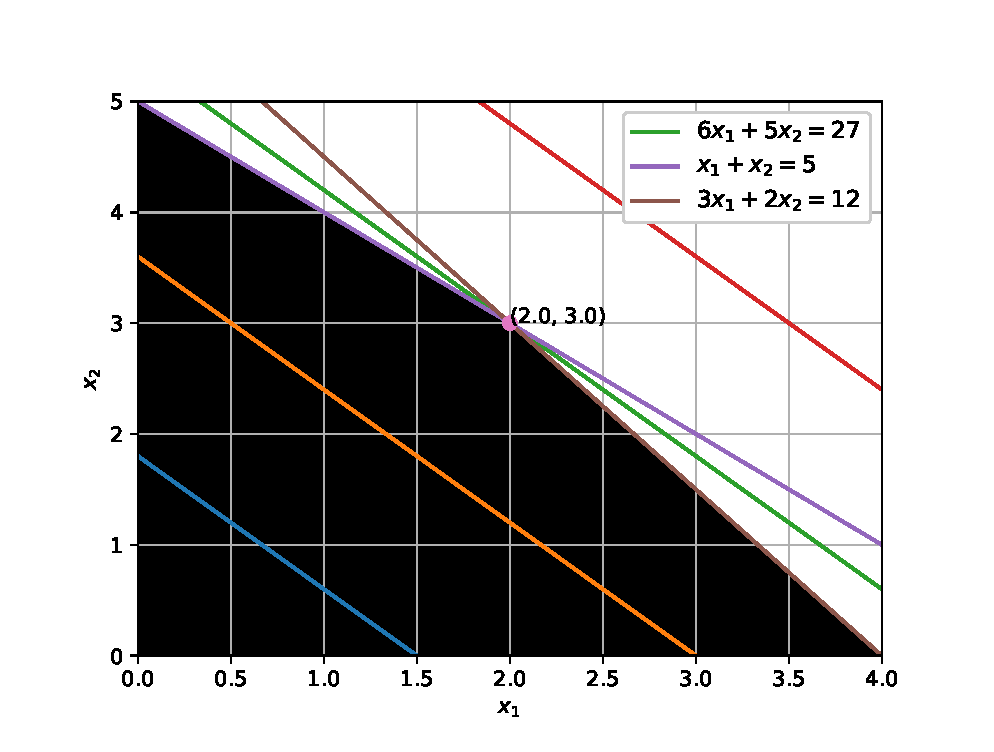
\includegraphics[width=\columnwidth]{./manual/figs/4.1.eps}
\caption{ The cost function intersects with the two constraints at $\mbf{x} = \brak{2,3}$. }
\label{fig.4.1}	
\end{figure}
%
\item
	Now use {\em cvxpy} to obtain a solution to problem \ref{ch1_lp1}.

\solution
The given problem is expressed as follows
%
\begin{align}
\min_{\mbf{x}}	\mbf{c}^{T}\mbf{x}\quad s.t.
\\
\mbf{A}\mbf{x} \preceq \mbf{b}
\end{align}
%
where
%
\begin{equation}
\mbf{c}
=
\begin{pmatrix}
-6
\\
-5
\end{pmatrix},
\mbf{A} = 
\begin{pmatrix}
1 & 1
\\
3 & 2
\\
-1 & 0
\\
0 & -1
\end{pmatrix},
\mbf{b}
= 
\begin{pmatrix}
5
\\
12
\\
0
\\
0 
\end{pmatrix}
\end{equation}
%	
The desired solution is then obtained using the following program.
%\begin{lstlisting}
%wget https://raw.githubusercontent.com/gadepall/optimization/master/manual/codes/4.2.py
%\end{lstlisting}
%
%
%\item
%Repeat the previous exercise using {\em cvxpy}
%
%\solution
\begin{lstlisting}
wget https://raw.githubusercontent.com/gadepall/optimization/master/manual/codes/4.2-cvx.py
\end{lstlisting}

\item
	Verify your solution to the above problem using the method of Lagrange multipliers.

%
\item
	 Maximise $5x_1 + 3x_2$ w.r.t the constraints
	 \begin{align}
	 x_1 + x_2 &\leq 2 \nonumber\\
	 5x_1 + 2x_2 &\leq 10 \nonumber\\
	 3x_1 + 8x_2 &\leq 12 \nonumber\\
	 \text{ where } x_1,x_2 &\geq 0 \nonumber
	 \end{align}	

\end{enumerate}
%
\section{Convex Polygon}
\begin{enumerate}[label=\thesection.\arabic*
,ref=\thesection.\theenumi]
\item Show that $\vec{D}$ lies inside $\triangle ABC$ iff
\begin{align}
\vec{D} = \lambda_1\vec{A} + \lambda_2\vec{B} + \lambda_3\vec{C}
\end{align}
such that
\begin{align}
0 \le \lambda_1, \lambda_2, \lambda_3 &\le 1,
\\
0 \le \lambda_1+\lambda_2+\lambda_3 &\le 1,
\end{align}
\item Prove that the point $\myvec{4\\4}$ lies outside the triangle whose sides are the lines
\begin{align}
\myvec{3&4} \vec{x}&= 24
\\
\myvec{ 5 & - 3} \vec{x}&= 15
\\
\myvec{0 &1} \vec{x}&= 0
\end{align}

\end{enumerate}
%
\section{Complex Numbers: Optimization}
\begin{enumerate}[label=\thesection.\arabic*
,ref=\thesection.\theenumi]
%
\item Consider the optimization problem
\begin{align}
\label{eq:opt_def}
\max_{z} \frac{1}{\abs{z-1}}
\\
s.t. \quad \abs{z-2 + \j} \ge \sqrt{5}
\end{align}
%
Show that it can be reframed as
\begin{align}
\label{eq:opt_rev}
\min_{\vec{x}} \,\norm{\vec{x} - \vec{c}_1}^2
\\
 s.t. \quad  \norm{\vec{x} - \vec{c}_2}^2 \ge 5
%\min_{z} \abs{z-1}
%\\
% s.t. \quad \abs{z-2 + \j} \ge \sqrt{5}
\end{align}
%
where
\begin{align}
z &= \vec{x} = \myvec{x_1 \\ x_2},
%\\
\vec{c}_1 = \myvec{1 \\ 0},
%\\
\vec{c}_2 = \myvec{2 \\ -1}
\end{align}

%
%
%Then, 
%\begin{align}
%\Gamma: \abs{z-1} = \norm{\vec{x} - \vec{c}_1}^2,
%\end{align}
%where 
%\begin{align}
%\end{align}
%Similarly, 
%\begin{align}
%\Omega:\abs{z-2+\j} = \norm{\vec{x} - \vec{c}_2}^2,
%\end{align}
%where 
%\begin{align}
%\end{align}
%
%Let 
%\begin{align}
% \abs{z_0-1} = r
%\end{align}
%
%
\item Explain the optimization problem with a figure.
\\
\solution
Fig. \ref{fig:2019_1} explains \eqref{eq:opt_rev}
where $z_0$ is the set of points comprising of the intersection of the 
smallest circle $\Gamma:$ with the largest circle $\Omega: r_2 \ge 
\sqrt{5}$ 
with radii 
$r_1$ and 
$r_2 \ge \sqrt{5}$ respectively.
\begin{figure}[!ht]
\centering
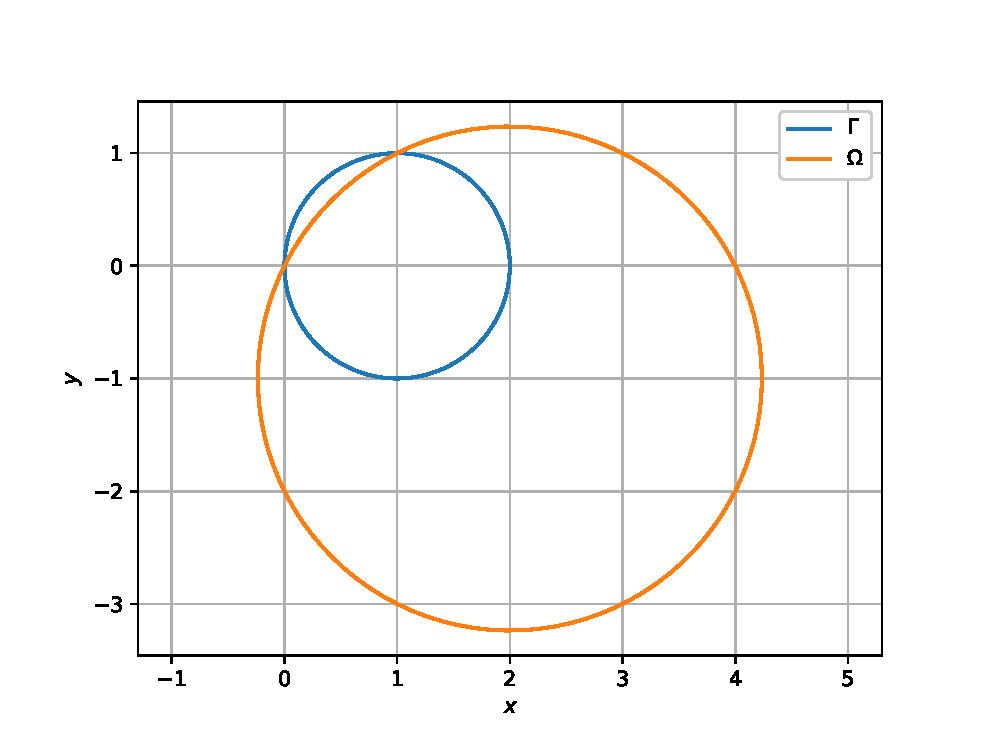
\includegraphics[width=\columnwidth]{./manual/figs/2019_1_1.eps}
\caption{}
\label{fig:2019_1}
\end{figure}
%
\item Obtain the Lagrangian.
\\
\solution
The Lagrangian is 
\begin{align}
L \brak{\vec{x},\lambda} = \norm{\vec{x} - \vec{c}_1}^2 - \lambda 
\cbrak{\norm{\vec{x} - \vec{c}_2}^2-r_2^2}
\end{align}
\item Use the KKT conditions to obtain the minima.
\\
\solution
From the KKT conditions, 
\begin{align}
\frac{\partial L \brak{\vec{x},\lambda}}{\partial \vec{x}} &= 0
\\
\implies {\vec{x} - \vec{c}_1} - \lambda \brak{\vec{x} - \vec{c}_2} &= 0
\\
\implies \vec{x}  = \frac{\vec{c}_1 -\lambda  \vec{c}_2}{1-\lambda } &
\label{eq:opt_xlam}
\end{align}
%
and 
\begin{align}
\frac{\partial L \brak{\vec{x},\lambda}}{\partial \lambda} &= 0
\\
\implies \norm{\vec{x} - \vec{c}_2}^2-r_2^2 &= 0
\label{eq:opt_xnorm}
\end{align}
Substituting from \eqref{eq:opt_xlam} in \eqref{eq:opt_xnorm},
\begin{align}
\norm{\frac{\vec{c}_1 -\lambda  \vec{c}_2}{1-\lambda } - \vec{c}_2}^2-r_2^2 &= 0
\\
\implies \lambda = 1\pm \frac{\norm{\vec{c}_1 - \vec{c}_2}}{r_2}&
\\
= 1 \pm \sqrt{\frac{2}{5}}
%\label{eq:opt_xnorm}
\end{align}
Fig. \ref{fig:2019_1_2} plots $\Gamma$ for 
\begin{align}
\lambda = 1 - \sqrt{\frac{2}{5}}
\end{align}
\item If the maximum value is obtained at $z_0$, find the principal argument of
\begin{align}
\frac{4 - z_0-\bar{z}_0}{z_0-\bar{z}_0+2\j}
\end{align}
\\
\solution 
From \eqref{eq:opt_xlam},
\begin{align}
 \vec{x}_0  &= \frac{\vec{c}_1 -\lambda  \vec{c}_2}{1-\lambda } 
\\
\implies z_0 &= \frac{1}{1-\lambda}\brak{1-2\lambda + \j \lambda }
\\
\text{or, }\arg \frac{4 - z_0-\bar{z}_0}{z_0-\bar{z}_0+2\j} &= \frac{2 - \Re\cbrak{z_0}}{\j\brak{\Im\cbrak{z_0}+1}}
\\
&=\frac{2\brak{1-\lambda}-\brak{1-2\lambda}}{\j} 
\\
&= -\j
\end{align}
%
Thus, the principal argument is $-\frac{\pi}{2}$.
\begin{figure}[!ht]
\centering
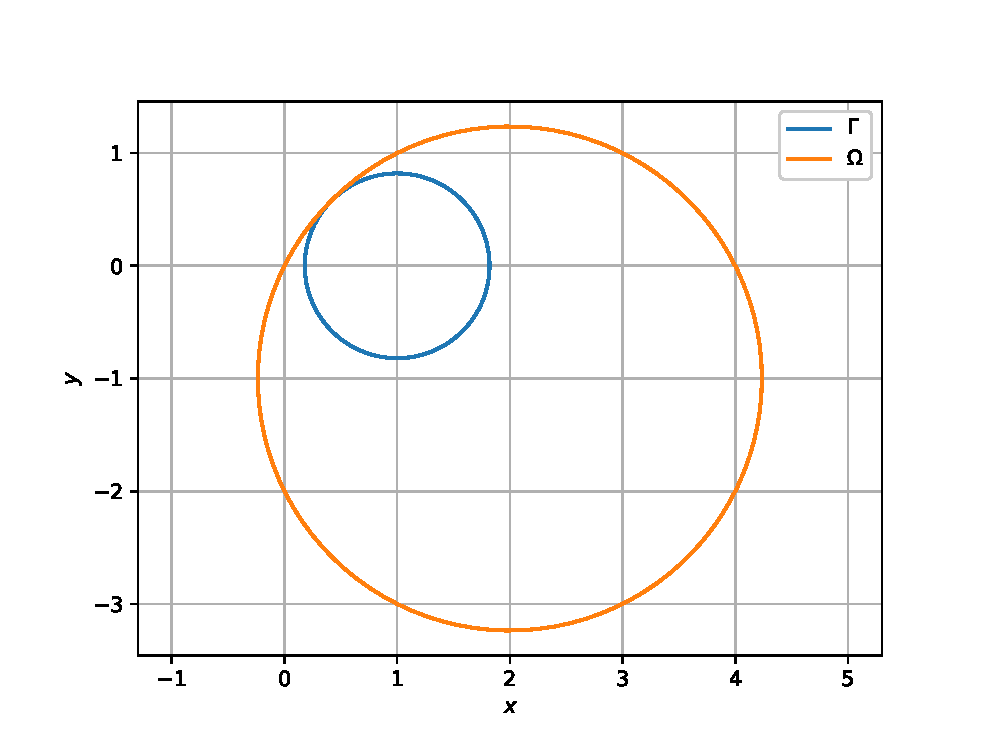
\includegraphics[width=\columnwidth]{./manual/figs/2019_1_2.eps}
\caption{}
\label{fig:2019_1_2}
\end{figure}

%\begin{enumerate}[label=\theenumi.\arabic*
%,ref=\thesection.\theenumi]
\item Show that the set 
\begin{align}
D = \cbrak{\vec{x}:\norm{\vec{x}-\vec{C}_2} \ge r_2}, r_2 > 0
\end{align}
%
is nonconvex.
\\
\solution Let $\vec{x}_1 \in D$ and 
\begin{align}
\vec{x}_2 = 2\vec{C}_2-\vec{x}_1
\end{align}
Then 
\begin{align}
\norm{\vec{x}_2-\vec{C}_2} &= \norm{\vec{C}_2-\vec{x}_1} \ge r_2
\\
\implies \vec{x}_2 &\in D.
\end{align}
Suppose 
\begin{align}
\vec{x} = \theta\vec{x}_1+\brak{1-\theta}\vec{x}_2
\end{align}
For $\theta = \frac{1}{2}$,
\begin{align}
\vec{x} &= \vec{C}_2
\\
\implies \norm{\vec{x}-\vec{C}_2} &= 0,
\\
\text{or, } \vec{x} &\notin D
\end{align}
Thus, by definition, $D$ is not a convex set.
\end{enumerate}

%\end{document}
\fi
